\documentclass{book}
\usepackage[a4paper,top=2.5cm,bottom=2.5cm,left=2.5cm,right=2.5cm]{geometry}
\usepackage{makeidx}
\usepackage{natbib}
\usepackage{graphicx}
\usepackage{multicol}
\usepackage{float}
\usepackage{listings}
\usepackage{color}
\usepackage{ifthen}
\usepackage[table]{xcolor}
\usepackage{textcomp}
\usepackage{alltt}
\usepackage{ifpdf}
\ifpdf
\usepackage[pdftex,
            pagebackref=true,
            colorlinks=true,
            linkcolor=blue,
            unicode
           ]{hyperref}
\else
\usepackage[ps2pdf,
            pagebackref=true,
            colorlinks=true,
            linkcolor=blue,
            unicode
           ]{hyperref}
\usepackage{pspicture}
\fi
\usepackage[utf8]{inputenc}
\usepackage[spanish]{babel}
\usepackage{mathptmx}
\usepackage[scaled=.90]{helvet}
\usepackage{courier}
\usepackage{sectsty}
\usepackage{amssymb}
\usepackage[titles]{tocloft}
\usepackage{doxygen}
\lstset{language=C++,inputencoding=utf8,basicstyle=\footnotesize,breaklines=true,breakatwhitespace=true,tabsize=2,numbers=left }
\makeindex
\setcounter{tocdepth}{3}
\renewcommand{\footrulewidth}{0.4pt}
\renewcommand{\familydefault}{\sfdefault}
\hfuzz=15pt
\setlength{\emergencystretch}{15pt}
\hbadness=750
\tolerance=750
\begin{document}
\hypersetup{pageanchor=false,citecolor=blue}
\begin{titlepage}
\vspace*{7cm}
\begin{center}
{\Large Gestor de tasques \\[1ex]\large version mayo-\/2015 }\\
\vspace*{1cm}
{\large Generado por Doxygen 1.8.3.1}\\
\vspace*{0.5cm}
{\small Lunes, 4 de Mayo de 2015 22:41:55}\\
\end{center}
\end{titlepage}
\clearemptydoublepage
\pagenumbering{roman}
\tableofcontents
\clearemptydoublepage
\pagenumbering{arabic}
\hypersetup{pageanchor=true,citecolor=blue}
\chapter{Índice de clases}
\section{Lista de clases}
Lista de las clases, estructuras, uniones e interfaces con una breve descripción\-:\begin{DoxyCompactList}
\item\contentsline{section}{\hyperlink{class_agenda}{Agenda} \\*Representa una colección de Tareas, ordenadas por la hora de tarea }{\pageref{class_agenda}}{}
\item\contentsline{section}{\hyperlink{class_comanda}{Comanda} \\*Representa una comanda (línia de text d'entrada). El mètode llegir permet utilitzar consultores sobre la comanda llegida i comprovar que no tingui errors sintàctics }{\pageref{class_comanda}}{}
\item\contentsline{section}{\hyperlink{class_reloj}{Reloj} }{\pageref{class_reloj}}{}
\item\contentsline{section}{\hyperlink{class_tags}{Tags} \\*Representa una colección de etiquetas }{\pageref{class_tags}}{}
\item\contentsline{section}{\hyperlink{class_tarea}{Tarea} }{\pageref{class_tarea}}{}
\item\contentsline{section}{\hyperlink{class_token}{Token} \\*Representa un string rellevant per a la classe \hyperlink{class_comanda}{Comanda} }{\pageref{class_token}}{}
\end{DoxyCompactList}

\chapter{Indice de archivos}
\section{Lista de archivos}
Lista de todos los archivos con descripciones breves\-:\begin{DoxyCompactList}
\item\contentsline{section}{\hyperlink{agenda_8hh}{agenda.\-hh} \\*Especificación de la clase \hyperlink{class_agenda}{Agenda} }{\pageref{agenda_8hh}}{}
\item\contentsline{section}{\hyperlink{comanda_8hh}{comanda.\-hh} \\*Classe \hyperlink{class_comanda}{Comanda} }{\pageref{comanda_8hh}}{}
\item\contentsline{section}{\hyperlink{reloj_8hh}{reloj.\-hh} \\*Clase \hyperlink{class_reloj}{Reloj} }{\pageref{reloj_8hh}}{}
\item\contentsline{section}{\hyperlink{tags_8hh}{tags.\-hh} \\*Especificación de la clase Tag }{\pageref{tags_8hh}}{}
\item\contentsline{section}{\hyperlink{tarea_8hh}{tarea.\-hh} }{\pageref{tarea_8hh}}{}
\item\contentsline{section}{\hyperlink{token_8hh}{token.\-hh} \\*Classe \hyperlink{class_token}{Token} }{\pageref{token_8hh}}{}
\end{DoxyCompactList}

\chapter{Documentación de las clases}
\hypertarget{class_agenda}{\section{Referencia de la Clase Agenda}
\label{class_agenda}\index{Agenda@{Agenda}}
}


Representa una colección de Tareas, ordenadas por la hora de tarea.  


\subsection*{Métodos públicos}
\begin{DoxyCompactItemize}
\item 
\hyperlink{class_agenda_a6685054d2b4ccbf2a4ef2ac5e3746bc3}{Agenda} ()
\begin{DoxyCompactList}\small\item\em Creadora por defecto. \end{DoxyCompactList}\item 
bool \hyperlink{class_agenda_a33563a51900832ac1daeeb3813d00fdc}{buscar\-\_\-tarea\-\_\-intervalo} (const \hyperlink{class_reloj}{Reloj} \&reloj1, const \hyperlink{class_reloj}{Reloj} \&reloj2, const string \&expr, map$<$ \hyperlink{class_reloj}{Reloj}, \hyperlink{class_tarea}{Tarea} $>$ \&map, bool excluir\-\_\-ultimo)
\begin{DoxyCompactList}\small\item\em Busca tareas en un intervalos y que cumplan una expresión. \end{DoxyCompactList}\item 
void \hyperlink{class_agenda_a02f25e376fa69a673fd4bf9349a033e1}{comprobar\-\_\-expr} (map$<$ \hyperlink{class_reloj}{Reloj}, \hyperlink{class_tarea}{Tarea} $>$ \&map, const string \&expr)
\begin{DoxyCompactList}\small\item\em borra todas las tareas que no cumplan la expresion, caso '$\ast$' no se borra nada \end{DoxyCompactList}\item 
void \hyperlink{class_agenda_a755177707be90968dedb6ff36647c3af}{imprimir\-\_\-menu} (const map$<$ \hyperlink{class_reloj}{Reloj}, \hyperlink{class_tarea}{Tarea} $>$ \&lista\-\_\-tareas)
\begin{DoxyCompactList}\small\item\em Imprime las tareas enumeradas. \end{DoxyCompactList}\item 
void \hyperlink{class_agenda_add9c46e874c521513328bee5c7fb7fee}{imprimir\-\_\-menu\-\_\-actual} ()
\begin{DoxyCompactList}\small\item\em Imprime todas las tareas que en el horario. \end{DoxyCompactList}\item 
bool \hyperlink{class_agenda_aeba776d0394a5cc0da53e7955d713133}{anadir\-\_\-tarea} (const \hyperlink{class_reloj}{Reloj} \&r, const \hyperlink{class_tarea}{Tarea} \&t)
\begin{DoxyCompactList}\small\item\em añade una tarea en la agenda \end{DoxyCompactList}\item 
bool \hyperlink{class_agenda_aecbb7c1af5d9816012ba9b6b7c5f3bfe}{modificar\-\_\-tarea} (const \hyperlink{class_reloj}{Reloj} \&reloj1, const \hyperlink{class_reloj}{Reloj} \&reloj2, const \hyperlink{class_tarea}{Tarea} \&t)
\begin{DoxyCompactList}\small\item\em modifica una tarea que hay en la agenda \end{DoxyCompactList}\item 
bool \hyperlink{class_agenda_aee3c8541a89cc0a52ea39efda99e52c8}{borrar\-\_\-tarea} (const \hyperlink{class_reloj}{Reloj} \&r)
\begin{DoxyCompactList}\small\item\em borra una tarea de la agenda \end{DoxyCompactList}\item 
\hyperlink{class_reloj}{Reloj} \hyperlink{class_agenda_afc5f9ca9546ff0000e4abe92584ac526}{consultar\-\_\-\-Reloj\-Actual} ()
\begin{DoxyCompactList}\small\item\em consulta la hora del reloj interno \end{DoxyCompactList}\item 
bool \hyperlink{class_agenda_a3c6df651d375edc2f3c2f06103eefd8b}{modificar\-\_\-\-Reloj\-Actual} (\hyperlink{class_reloj}{Reloj} r)
\begin{DoxyCompactList}\small\item\em modifica la hora del reloj interno \end{DoxyCompactList}\end{DoxyCompactItemize}


\subsection{Descripción detallada}
Representa una colección de Tareas, ordenadas por la hora de tarea. 

Definición en la línea 16 del archivo agenda.\-hh.



\subsection{Documentación del constructor y destructor}
\hypertarget{class_agenda_a6685054d2b4ccbf2a4ef2ac5e3746bc3}{\index{Agenda@{Agenda}!Agenda@{Agenda}}
\index{Agenda@{Agenda}!Agenda@{Agenda}}
\subsubsection[{Agenda}]{\setlength{\rightskip}{0pt plus 5cm}Agenda\-::\-Agenda (
\begin{DoxyParamCaption}
{}
\end{DoxyParamCaption}
)}}\label{class_agenda_a6685054d2b4ccbf2a4ef2ac5e3746bc3}


Creadora por defecto. 

Se ejecuta automáticamente al declarar una agenda

\begin{DoxyPrecond}{Precondición}
cierto 
\end{DoxyPrecond}
\begin{DoxyPostcond}{Postcondición}
el resultado es una agenta sin tareas y con el reloj actual a a 20/04/15 00\-:00 
\end{DoxyPostcond}


\subsection{Documentación de las funciones miembro}
\hypertarget{class_agenda_a33563a51900832ac1daeeb3813d00fdc}{\index{Agenda@{Agenda}!buscar\-\_\-tarea\-\_\-intervalo@{buscar\-\_\-tarea\-\_\-intervalo}}
\index{buscar\-\_\-tarea\-\_\-intervalo@{buscar\-\_\-tarea\-\_\-intervalo}!Agenda@{Agenda}}
\subsubsection[{buscar\-\_\-tarea\-\_\-intervalo}]{\setlength{\rightskip}{0pt plus 5cm}bool Agenda\-::buscar\-\_\-tarea\-\_\-intervalo (
\begin{DoxyParamCaption}
\item[{const {\bf Reloj} \&}]{reloj1, }
\item[{const {\bf Reloj} \&}]{reloj2, }
\item[{const string \&}]{expr, }
\item[{map$<$ {\bf Reloj}, {\bf Tarea} $>$ \&}]{map, }
\item[{bool}]{excluir\-\_\-ultimo}
\end{DoxyParamCaption}
)}}\label{class_agenda_a33563a51900832ac1daeeb3813d00fdc}


Busca tareas en un intervalos y que cumplan una expresión. 

\begin{DoxyPrecond}{Precondición}
{\itshape reloj1} $<$ {\itshape reloj2} y {\itshape expr} es una string que puede ser '$\ast$' en caso de que no tenga ninguna condición sobre etiquetas, '\#$<$etiqueta$>$' donde hay una sola etiqueta para buscar o el string contenga una expresion con condiciones A\-N\-D y O\-R. 
\end{DoxyPrecond}
\begin{DoxyPostcond}{Postcondición}
El resultado es un map$<$\-Reloj,\-Tarea$>$ donde están todas las tareas que hay en ese intervalo y que cumpla la expresión y excluyendo el ultimo elemento si el excluir\-\_\-ultimo es cierto 
\end{DoxyPostcond}
\hypertarget{class_agenda_a02f25e376fa69a673fd4bf9349a033e1}{\index{Agenda@{Agenda}!comprobar\-\_\-expr@{comprobar\-\_\-expr}}
\index{comprobar\-\_\-expr@{comprobar\-\_\-expr}!Agenda@{Agenda}}
\subsubsection[{comprobar\-\_\-expr}]{\setlength{\rightskip}{0pt plus 5cm}void Agenda\-::comprobar\-\_\-expr (
\begin{DoxyParamCaption}
\item[{map$<$ {\bf Reloj}, {\bf Tarea} $>$ \&}]{map, }
\item[{const string \&}]{expr}
\end{DoxyParamCaption}
)}}\label{class_agenda_a02f25e376fa69a673fd4bf9349a033e1}


borra todas las tareas que no cumplan la expresion, caso '$\ast$' no se borra nada 

\begin{DoxyPrecond}{Precondición}
{\itshape expr} es un exprecion bien hecha o es un '$\ast$' 
\end{DoxyPrecond}
\begin{DoxyPostcond}{Postcondición}
modifica el {\itshape map} borrando las tareas que no cumplan la expresion 
\end{DoxyPostcond}
\hypertarget{class_agenda_a755177707be90968dedb6ff36647c3af}{\index{Agenda@{Agenda}!imprimir\-\_\-menu@{imprimir\-\_\-menu}}
\index{imprimir\-\_\-menu@{imprimir\-\_\-menu}!Agenda@{Agenda}}
\subsubsection[{imprimir\-\_\-menu}]{\setlength{\rightskip}{0pt plus 5cm}void Agenda\-::imprimir\-\_\-menu (
\begin{DoxyParamCaption}
\item[{const map$<$ {\bf Reloj}, {\bf Tarea} $>$ \&}]{lista\-\_\-tareas}
\end{DoxyParamCaption}
)}}\label{class_agenda_a755177707be90968dedb6ff36647c3af}


Imprime las tareas enumeradas. 

\begin{DoxyPrecond}{Precondición}
cierto 
\end{DoxyPrecond}
\begin{DoxyPostcond}{Postcondición}
cierto 
\end{DoxyPostcond}
\hypertarget{class_agenda_add9c46e874c521513328bee5c7fb7fee}{\index{Agenda@{Agenda}!imprimir\-\_\-menu\-\_\-actual@{imprimir\-\_\-menu\-\_\-actual}}
\index{imprimir\-\_\-menu\-\_\-actual@{imprimir\-\_\-menu\-\_\-actual}!Agenda@{Agenda}}
\subsubsection[{imprimir\-\_\-menu\-\_\-actual}]{\setlength{\rightskip}{0pt plus 5cm}void Agenda\-::imprimir\-\_\-menu\-\_\-actual (
\begin{DoxyParamCaption}
{}
\end{DoxyParamCaption}
)}}\label{class_agenda_add9c46e874c521513328bee5c7fb7fee}


Imprime todas las tareas que en el horario. 

\begin{DoxyPrecond}{Precondición}
horario no vaio 
\end{DoxyPrecond}
\begin{DoxyPostcond}{Postcondición}
cierto 
\end{DoxyPostcond}
\hypertarget{class_agenda_aeba776d0394a5cc0da53e7955d713133}{\index{Agenda@{Agenda}!anadir\-\_\-tarea@{anadir\-\_\-tarea}}
\index{anadir\-\_\-tarea@{anadir\-\_\-tarea}!Agenda@{Agenda}}
\subsubsection[{anadir\-\_\-tarea}]{\setlength{\rightskip}{0pt plus 5cm}bool Agenda\-::anadir\-\_\-tarea (
\begin{DoxyParamCaption}
\item[{const {\bf Reloj} \&}]{r, }
\item[{const {\bf Tarea} \&}]{t}
\end{DoxyParamCaption}
)}}\label{class_agenda_aeba776d0394a5cc0da53e7955d713133}


añade una tarea en la agenda 

\begin{DoxyPrecond}{Precondición}
cierto 
\end{DoxyPrecond}
\begin{DoxyPostcond}{Postcondición}
devuelve true si se ha podido añadir y en caso contrario vuelve false 
\end{DoxyPostcond}
\hypertarget{class_agenda_aecbb7c1af5d9816012ba9b6b7c5f3bfe}{\index{Agenda@{Agenda}!modificar\-\_\-tarea@{modificar\-\_\-tarea}}
\index{modificar\-\_\-tarea@{modificar\-\_\-tarea}!Agenda@{Agenda}}
\subsubsection[{modificar\-\_\-tarea}]{\setlength{\rightskip}{0pt plus 5cm}bool Agenda\-::modificar\-\_\-tarea (
\begin{DoxyParamCaption}
\item[{const {\bf Reloj} \&}]{reloj1, }
\item[{const {\bf Reloj} \&}]{reloj2, }
\item[{const {\bf Tarea} \&}]{t}
\end{DoxyParamCaption}
)}}\label{class_agenda_aecbb7c1af5d9816012ba9b6b7c5f3bfe}


modifica una tarea que hay en la agenda 

\begin{DoxyPrecond}{Precondición}
la tarea ya este en la agenda, si no se cambia la fecha y hora {\itshape reloj1} es igual a {\itshape reloj2} y {\itshape reloj1} tienes que ser el reloj original y {\itshape reloj2} el reloj cambiado 
\end{DoxyPrecond}
\begin{DoxyPostcond}{Postcondición}
devuelve true si se ha podido modificar en caso contrtio se devuelve falso 
\end{DoxyPostcond}
\hypertarget{class_agenda_aee3c8541a89cc0a52ea39efda99e52c8}{\index{Agenda@{Agenda}!borrar\-\_\-tarea@{borrar\-\_\-tarea}}
\index{borrar\-\_\-tarea@{borrar\-\_\-tarea}!Agenda@{Agenda}}
\subsubsection[{borrar\-\_\-tarea}]{\setlength{\rightskip}{0pt plus 5cm}bool Agenda\-::borrar\-\_\-tarea (
\begin{DoxyParamCaption}
\item[{const {\bf Reloj} \&}]{r}
\end{DoxyParamCaption}
)}}\label{class_agenda_aee3c8541a89cc0a52ea39efda99e52c8}


borra una tarea de la agenda 

\begin{DoxyPrecond}{Precondición}
La tarea esta en la agenda 
\end{DoxyPrecond}
\begin{DoxyPostcond}{Postcondición}
devuelve true si se ha podido borrar la tarea de la agenda 
\end{DoxyPostcond}
\hypertarget{class_agenda_afc5f9ca9546ff0000e4abe92584ac526}{\index{Agenda@{Agenda}!consultar\-\_\-\-Reloj\-Actual@{consultar\-\_\-\-Reloj\-Actual}}
\index{consultar\-\_\-\-Reloj\-Actual@{consultar\-\_\-\-Reloj\-Actual}!Agenda@{Agenda}}
\subsubsection[{consultar\-\_\-\-Reloj\-Actual}]{\setlength{\rightskip}{0pt plus 5cm}{\bf Reloj} Agenda\-::consultar\-\_\-\-Reloj\-Actual (
\begin{DoxyParamCaption}
{}
\end{DoxyParamCaption}
)}}\label{class_agenda_afc5f9ca9546ff0000e4abe92584ac526}


consulta la hora del reloj interno 

\begin{DoxyPrecond}{Precondición}
cierto 
\end{DoxyPrecond}
\begin{DoxyPostcond}{Postcondición}
devuelve la hora interna del reloj 
\end{DoxyPostcond}
\hypertarget{class_agenda_a3c6df651d375edc2f3c2f06103eefd8b}{\index{Agenda@{Agenda}!modificar\-\_\-\-Reloj\-Actual@{modificar\-\_\-\-Reloj\-Actual}}
\index{modificar\-\_\-\-Reloj\-Actual@{modificar\-\_\-\-Reloj\-Actual}!Agenda@{Agenda}}
\subsubsection[{modificar\-\_\-\-Reloj\-Actual}]{\setlength{\rightskip}{0pt plus 5cm}bool Agenda\-::modificar\-\_\-\-Reloj\-Actual (
\begin{DoxyParamCaption}
\item[{{\bf Reloj}}]{r}
\end{DoxyParamCaption}
)}}\label{class_agenda_a3c6df651d375edc2f3c2f06103eefd8b}


modifica la hora del reloj interno 

\begin{DoxyPrecond}{Precondición}
cierto 
\end{DoxyPrecond}
\begin{DoxyPostcond}{Postcondición}
devuelve true si se ha modificado el reloj interno 
\end{DoxyPostcond}


La documentación para esta clase fue generada a partir del siguiente fichero\-:\begin{DoxyCompactItemize}
\item 
\hyperlink{agenda_8hh}{agenda.\-hh}\end{DoxyCompactItemize}

\hypertarget{class_comanda}{\section{Referencia de la Clase Comanda}
\label{class_comanda}\index{Comanda@{Comanda}}
}


Representa una comanda (línia de text d'entrada). El mètode llegir permet utilitzar consultores sobre la comanda llegida i comprovar que no tingui errors sintàctics.  


\subsection*{Métodos públicos}
\begin{DoxyCompactItemize}
\item 
\hyperlink{class_comanda_a0f09e7aa5b7c15f131020d04bf5a8a94}{Comanda} ()
\item 
bool \hyperlink{class_comanda_af2dbc8ccdbb94bed6ea26155edc71b57}{llegir} (bool \&be)
\begin{DoxyCompactList}\small\item\em Llegeix una comanda (línia de text d'entrada) i actualitza la informació interna perquè funcionin bé les consultores. \end{DoxyCompactList}\item 
bool \hyperlink{class_comanda_a614467bedacc9cf29cc5a9dcbba6b23d}{es\-\_\-insercio} ()
\begin{DoxyCompactList}\small\item\em Comprova si la comanda és una inserció (\char`\"{}+\char`\"{} és el primer string) \end{DoxyCompactList}\item 
bool \hyperlink{class_comanda_a847ee227fd7fea3a105dbd78735de453}{es\-\_\-consulta} ()
\begin{DoxyCompactList}\small\item\em Comprova si la comanda és una consulta (\char`\"{}?\char`\"{}, \char`\"{}passat?\char`\"{} o \char`\"{}rellotge?\char`\"{} és el primer string) \end{DoxyCompactList}\item 
bool \hyperlink{class_comanda_a1f435f8b605f0d1f5cbb06c8c6fe4005}{es\-\_\-passat} ()
\begin{DoxyCompactList}\small\item\em Comprova si la comanda és una consulta del passat (\char`\"{}passat?\char`\"{} és el primer string) \end{DoxyCompactList}\item 
bool \hyperlink{class_comanda_a2a33a5497c7d156f22065656cb48d9a1}{es\-\_\-modificacio} ()
\begin{DoxyCompactList}\small\item\em Comprova si la comanda és una modificació (el primer string és un enter, però el segon no comença per \char`\"{}-\/\char`\"{}) \end{DoxyCompactList}\item 
bool \hyperlink{class_comanda_aa8767f298317c3bb07f90676cabb8c43}{es\-\_\-rellotge} ()
\begin{DoxyCompactList}\small\item\em Comprova si la comanda és sobre el rellotge (el primer string és \char`\"{}rellotge\char`\"{} o \char`\"{}rellotge?\char`\"{}) \end{DoxyCompactList}\item 
bool \hyperlink{class_comanda_a9e71320e8617ce224c8d994d0969555a}{es\-\_\-esborrat} ()
\begin{DoxyCompactList}\small\item\em Comprova si la comanda és d'esborrat (comença per \char`\"{}-\/k\char`\"{} o per \char`\"{}k -\/x\char`\"{}, on k és un enter) \end{DoxyCompactList}\item 
string \hyperlink{class_comanda_a998dc172668a108837512f818ca5430f}{tipus\-\_\-esborrat} ()
\begin{DoxyCompactList}\small\item\em Consulta el tipus d'esborrat. \end{DoxyCompactList}\item 
int \hyperlink{class_comanda_aadabfc85ec7cdeb45039e8952a1ab124}{nombre\-\_\-dates} ()
\begin{DoxyCompactList}\small\item\em Consulta el nombre de dates contingudes en la comanda. \end{DoxyCompactList}\item 
string \hyperlink{class_comanda_ab4ce0a50bde32145d11cbaee753526c7}{data} (int i)
\begin{DoxyCompactList}\small\item\em Consulta una data individual de la comanda. \end{DoxyCompactList}\item 
bool \hyperlink{class_comanda_abf8b926146f3664aacfd24d7800014e5}{te\-\_\-hora} ()
\begin{DoxyCompactList}\small\item\em Comprova si la comanda conté hora. \end{DoxyCompactList}\item 
string \hyperlink{class_comanda_ae8bca2ad702d3316dc1c53dcab7cac02}{hora} ()
\begin{DoxyCompactList}\small\item\em Consulta l'hora de la comanda. \end{DoxyCompactList}\item 
bool \hyperlink{class_comanda_a5452f5a877d58627cd2bd871cf31b074}{te\-\_\-titol} ()
\begin{DoxyCompactList}\small\item\em Comprova si la comanda conté un títol (una seqüència de paraules, és a dir, strings que comencen per una lletra i no contenen ni \char`\"{}.\char`\"{} ni \char`\"{},\char`\"{} ni \char`\"{}\-:\char`\"{} ni \char`\"{}\#\char`\"{}) \end{DoxyCompactList}\item 
string \hyperlink{class_comanda_ad1cefdda3db389d9ab536a59e2ee907d}{titol} ()
\begin{DoxyCompactList}\small\item\em Consulta el títol de la comanda. \end{DoxyCompactList}\item 
int \hyperlink{class_comanda_a4280b6ae2d435d9c21bbed364cb1db3d}{nombre\-\_\-etiquetes} ()
\begin{DoxyCompactList}\small\item\em Consulta el nombre d'etiquetes de la comanda (strings que comencen per \# seguit d'una paraula) \end{DoxyCompactList}\item 
string \hyperlink{class_comanda_ac80e9a80d16c6bac9a134e431bca1ed0}{etiqueta} (int i)
\begin{DoxyCompactList}\small\item\em Consulta una etiqueta de la comanda. \end{DoxyCompactList}\item 
bool \hyperlink{class_comanda_a81d17f4233e33f3baac7633546c066f0}{te\-\_\-expressio} ()
\begin{DoxyCompactList}\small\item\em Consulta la presència d'una expressió booleana d'etiquetes en la comanda, és a dir, una expressió ben parentitzada, on els operadors són \char`\"{},\char`\"{} (disjunció binària) i \char`\"{}.\char`\"{} (conjunció binària) i els operands són etiquetes. \end{DoxyCompactList}\item 
string \hyperlink{class_comanda_aa3191131592fbf58d20bed1052c31cd1}{expressio} ()
\begin{DoxyCompactList}\small\item\em Consulta una expressió d'etiquetes. \end{DoxyCompactList}\item 
int \hyperlink{class_comanda_a67591051e9c5977c324ad8f8c3ac16e3}{tasca} ()
\begin{DoxyCompactList}\small\item\em Consulta el número de tasca que hi ha a la comanda. \end{DoxyCompactList}\end{DoxyCompactItemize}


\subsection{Descripción detallada}
Representa una comanda (línia de text d'entrada). El mètode llegir permet utilitzar consultores sobre la comanda llegida i comprovar que no tingui errors sintàctics. 

Definición en la línea 21 del archivo comanda.\-hh.



\subsection{Documentación del constructor y destructor}
\hypertarget{class_comanda_a0f09e7aa5b7c15f131020d04bf5a8a94}{\index{Comanda@{Comanda}!Comanda@{Comanda}}
\index{Comanda@{Comanda}!Comanda@{Comanda}}
\subsubsection[{Comanda}]{\setlength{\rightskip}{0pt plus 5cm}Comanda\-::\-Comanda (
\begin{DoxyParamCaption}
{}
\end{DoxyParamCaption}
)}}\label{class_comanda_a0f09e7aa5b7c15f131020d04bf5a8a94}


\subsection{Documentación de las funciones miembro}
\hypertarget{class_comanda_af2dbc8ccdbb94bed6ea26155edc71b57}{\index{Comanda@{Comanda}!llegir@{llegir}}
\index{llegir@{llegir}!Comanda@{Comanda}}
\subsubsection[{llegir}]{\setlength{\rightskip}{0pt plus 5cm}bool Comanda\-::llegir (
\begin{DoxyParamCaption}
\item[{bool \&}]{be}
\end{DoxyParamCaption}
)}}\label{class_comanda_af2dbc8ccdbb94bed6ea26155edc71b57}


Llegeix una comanda (línia de text d'entrada) i actualitza la informació interna perquè funcionin bé les consultores. 

\begin{DoxyPrecond}{Precondición}
cert 
\end{DoxyPrecond}
\begin{DoxyPostcond}{Postcondición}
si s'ha llegit una comanda sense errors sintàctics, be = cert i s'escriu la comanda; si la comanda té errors sintàctics, be = fals i s'escriu \char`\"{}\-Error de format\char`\"{}; retorna cert quan la comanda no és \char`\"{}sortir\char`\"{} 
\end{DoxyPostcond}
\hypertarget{class_comanda_a614467bedacc9cf29cc5a9dcbba6b23d}{\index{Comanda@{Comanda}!es\-\_\-insercio@{es\-\_\-insercio}}
\index{es\-\_\-insercio@{es\-\_\-insercio}!Comanda@{Comanda}}
\subsubsection[{es\-\_\-insercio}]{\setlength{\rightskip}{0pt plus 5cm}bool Comanda\-::es\-\_\-insercio (
\begin{DoxyParamCaption}
{}
\end{DoxyParamCaption}
)}}\label{class_comanda_a614467bedacc9cf29cc5a9dcbba6b23d}


Comprova si la comanda és una inserció (\char`\"{}+\char`\"{} és el primer string) 

\begin{DoxyPrecond}{Precondición}
\-: cert 
\end{DoxyPrecond}
\begin{DoxyPostcond}{Postcondición}
\-: cert si és una inserció 
\end{DoxyPostcond}
\hypertarget{class_comanda_a847ee227fd7fea3a105dbd78735de453}{\index{Comanda@{Comanda}!es\-\_\-consulta@{es\-\_\-consulta}}
\index{es\-\_\-consulta@{es\-\_\-consulta}!Comanda@{Comanda}}
\subsubsection[{es\-\_\-consulta}]{\setlength{\rightskip}{0pt plus 5cm}bool Comanda\-::es\-\_\-consulta (
\begin{DoxyParamCaption}
{}
\end{DoxyParamCaption}
)}}\label{class_comanda_a847ee227fd7fea3a105dbd78735de453}


Comprova si la comanda és una consulta (\char`\"{}?\char`\"{}, \char`\"{}passat?\char`\"{} o \char`\"{}rellotge?\char`\"{} és el primer string) 

\begin{DoxyPrecond}{Precondición}
cert 
\end{DoxyPrecond}
\begin{DoxyPostcond}{Postcondición}
cert si és una consulta 
\end{DoxyPostcond}
\hypertarget{class_comanda_a1f435f8b605f0d1f5cbb06c8c6fe4005}{\index{Comanda@{Comanda}!es\-\_\-passat@{es\-\_\-passat}}
\index{es\-\_\-passat@{es\-\_\-passat}!Comanda@{Comanda}}
\subsubsection[{es\-\_\-passat}]{\setlength{\rightskip}{0pt plus 5cm}bool Comanda\-::es\-\_\-passat (
\begin{DoxyParamCaption}
{}
\end{DoxyParamCaption}
)}}\label{class_comanda_a1f435f8b605f0d1f5cbb06c8c6fe4005}


Comprova si la comanda és una consulta del passat (\char`\"{}passat?\char`\"{} és el primer string) 

\begin{DoxyPrecond}{Precondición}
cert 
\end{DoxyPrecond}
\begin{DoxyPostcond}{Postcondición}
cert si és una consulta sobre el passat 
\end{DoxyPostcond}
\hypertarget{class_comanda_a2a33a5497c7d156f22065656cb48d9a1}{\index{Comanda@{Comanda}!es\-\_\-modificacio@{es\-\_\-modificacio}}
\index{es\-\_\-modificacio@{es\-\_\-modificacio}!Comanda@{Comanda}}
\subsubsection[{es\-\_\-modificacio}]{\setlength{\rightskip}{0pt plus 5cm}bool Comanda\-::es\-\_\-modificacio (
\begin{DoxyParamCaption}
{}
\end{DoxyParamCaption}
)}}\label{class_comanda_a2a33a5497c7d156f22065656cb48d9a1}


Comprova si la comanda és una modificació (el primer string és un enter, però el segon no comença per \char`\"{}-\/\char`\"{}) 

\begin{DoxyPrecond}{Precondición}
cert 
\end{DoxyPrecond}
\begin{DoxyPostcond}{Postcondición}
cert si és una modificació 
\end{DoxyPostcond}
\hypertarget{class_comanda_aa8767f298317c3bb07f90676cabb8c43}{\index{Comanda@{Comanda}!es\-\_\-rellotge@{es\-\_\-rellotge}}
\index{es\-\_\-rellotge@{es\-\_\-rellotge}!Comanda@{Comanda}}
\subsubsection[{es\-\_\-rellotge}]{\setlength{\rightskip}{0pt plus 5cm}bool Comanda\-::es\-\_\-rellotge (
\begin{DoxyParamCaption}
{}
\end{DoxyParamCaption}
)}}\label{class_comanda_aa8767f298317c3bb07f90676cabb8c43}


Comprova si la comanda és sobre el rellotge (el primer string és \char`\"{}rellotge\char`\"{} o \char`\"{}rellotge?\char`\"{}) 

\begin{DoxyPrecond}{Precondición}
cert 
\end{DoxyPrecond}
\begin{DoxyPostcond}{Postcondición}
cert si la comanda és una consulta sobre el rellotge o una modificació del temps del rellotge 
\end{DoxyPostcond}
\hypertarget{class_comanda_a9e71320e8617ce224c8d994d0969555a}{\index{Comanda@{Comanda}!es\-\_\-esborrat@{es\-\_\-esborrat}}
\index{es\-\_\-esborrat@{es\-\_\-esborrat}!Comanda@{Comanda}}
\subsubsection[{es\-\_\-esborrat}]{\setlength{\rightskip}{0pt plus 5cm}bool Comanda\-::es\-\_\-esborrat (
\begin{DoxyParamCaption}
{}
\end{DoxyParamCaption}
)}}\label{class_comanda_a9e71320e8617ce224c8d994d0969555a}


Comprova si la comanda és d'esborrat (comença per \char`\"{}-\/k\char`\"{} o per \char`\"{}k -\/x\char`\"{}, on k és un enter) 

\begin{DoxyPrecond}{Precondición}
cert 
\end{DoxyPrecond}
\begin{DoxyPostcond}{Postcondición}
cert si és un esborrat 
\end{DoxyPostcond}
\hypertarget{class_comanda_a998dc172668a108837512f818ca5430f}{\index{Comanda@{Comanda}!tipus\-\_\-esborrat@{tipus\-\_\-esborrat}}
\index{tipus\-\_\-esborrat@{tipus\-\_\-esborrat}!Comanda@{Comanda}}
\subsubsection[{tipus\-\_\-esborrat}]{\setlength{\rightskip}{0pt plus 5cm}string Comanda\-::tipus\-\_\-esborrat (
\begin{DoxyParamCaption}
{}
\end{DoxyParamCaption}
)}}\label{class_comanda_a998dc172668a108837512f818ca5430f}


Consulta el tipus d'esborrat. 

\begin{DoxyPrecond}{Precondición}
la comanda és d'esborrat 
\end{DoxyPrecond}
\begin{DoxyPostcond}{Postcondición}
retorna el tipus d'esborrat\-: \char`\"{}etiquetes\char`\"{} (si cal esborrar totes les etiquetes), \char`\"{}etiqueta\char`\"{} (si cal esborrar-\/ne una) o \char`\"{}tasca\char`\"{} (si cal esborrar la tasca) 
\end{DoxyPostcond}
\hypertarget{class_comanda_aadabfc85ec7cdeb45039e8952a1ab124}{\index{Comanda@{Comanda}!nombre\-\_\-dates@{nombre\-\_\-dates}}
\index{nombre\-\_\-dates@{nombre\-\_\-dates}!Comanda@{Comanda}}
\subsubsection[{nombre\-\_\-dates}]{\setlength{\rightskip}{0pt plus 5cm}int Comanda\-::nombre\-\_\-dates (
\begin{DoxyParamCaption}
{}
\end{DoxyParamCaption}
)}}\label{class_comanda_aadabfc85ec7cdeb45039e8952a1ab124}


Consulta el nombre de dates contingudes en la comanda. 

\begin{DoxyPrecond}{Precondición}
cert 
\end{DoxyPrecond}
\begin{DoxyPostcond}{Postcondición}
retorna el nombre de dates proporcionades en la comanda (0, 1 o 2) 
\end{DoxyPostcond}
\hypertarget{class_comanda_ab4ce0a50bde32145d11cbaee753526c7}{\index{Comanda@{Comanda}!data@{data}}
\index{data@{data}!Comanda@{Comanda}}
\subsubsection[{data}]{\setlength{\rightskip}{0pt plus 5cm}string Comanda\-::data (
\begin{DoxyParamCaption}
\item[{int}]{i}
\end{DoxyParamCaption}
)}}\label{class_comanda_ab4ce0a50bde32145d11cbaee753526c7}


Consulta una data individual de la comanda. 

\begin{DoxyPrecond}{Precondición}
1 $<$= i $<$= \hyperlink{class_comanda_aadabfc85ec7cdeb45039e8952a1ab124}{nombre\-\_\-dates()} 
\end{DoxyPrecond}
\begin{DoxyPostcond}{Postcondición}
retorna la data i-\/èsima de la comanda 
\end{DoxyPostcond}
\hypertarget{class_comanda_abf8b926146f3664aacfd24d7800014e5}{\index{Comanda@{Comanda}!te\-\_\-hora@{te\-\_\-hora}}
\index{te\-\_\-hora@{te\-\_\-hora}!Comanda@{Comanda}}
\subsubsection[{te\-\_\-hora}]{\setlength{\rightskip}{0pt plus 5cm}bool Comanda\-::te\-\_\-hora (
\begin{DoxyParamCaption}
{}
\end{DoxyParamCaption}
)}}\label{class_comanda_abf8b926146f3664aacfd24d7800014e5}


Comprova si la comanda conté hora. 

\begin{DoxyPrecond}{Precondición}
cert 
\end{DoxyPrecond}
\begin{DoxyPostcond}{Postcondición}
cert si la comanda conté hora 
\end{DoxyPostcond}
\hypertarget{class_comanda_ae8bca2ad702d3316dc1c53dcab7cac02}{\index{Comanda@{Comanda}!hora@{hora}}
\index{hora@{hora}!Comanda@{Comanda}}
\subsubsection[{hora}]{\setlength{\rightskip}{0pt plus 5cm}string Comanda\-::hora (
\begin{DoxyParamCaption}
{}
\end{DoxyParamCaption}
)}}\label{class_comanda_ae8bca2ad702d3316dc1c53dcab7cac02}


Consulta l'hora de la comanda. 

\begin{DoxyPrecond}{Precondición}
la comanda conté hora 
\end{DoxyPrecond}
\begin{DoxyPostcond}{Postcondición}
retorna l'hora continguda en la comanda 
\end{DoxyPostcond}
\hypertarget{class_comanda_a5452f5a877d58627cd2bd871cf31b074}{\index{Comanda@{Comanda}!te\-\_\-titol@{te\-\_\-titol}}
\index{te\-\_\-titol@{te\-\_\-titol}!Comanda@{Comanda}}
\subsubsection[{te\-\_\-titol}]{\setlength{\rightskip}{0pt plus 5cm}bool Comanda\-::te\-\_\-titol (
\begin{DoxyParamCaption}
{}
\end{DoxyParamCaption}
)}}\label{class_comanda_a5452f5a877d58627cd2bd871cf31b074}


Comprova si la comanda conté un títol (una seqüència de paraules, és a dir, strings que comencen per una lletra i no contenen ni \char`\"{}.\char`\"{} ni \char`\"{},\char`\"{} ni \char`\"{}\-:\char`\"{} ni \char`\"{}\#\char`\"{}) 

\begin{DoxyPrecond}{Precondición}
cert 
\end{DoxyPrecond}
\begin{DoxyPostcond}{Postcondición}
retorna cert si la comanda conté un títol 
\end{DoxyPostcond}
\hypertarget{class_comanda_ad1cefdda3db389d9ab536a59e2ee907d}{\index{Comanda@{Comanda}!titol@{titol}}
\index{titol@{titol}!Comanda@{Comanda}}
\subsubsection[{titol}]{\setlength{\rightskip}{0pt plus 5cm}string Comanda\-::titol (
\begin{DoxyParamCaption}
{}
\end{DoxyParamCaption}
)}}\label{class_comanda_ad1cefdda3db389d9ab536a59e2ee907d}


Consulta el títol de la comanda. 

\begin{DoxyPrecond}{Precondición}
és una inserció o és una modificació amb títol 
\end{DoxyPrecond}
\begin{DoxyPostcond}{Postcondición}
retorna el títol contingut en la comanda 
\end{DoxyPostcond}
\hypertarget{class_comanda_a4280b6ae2d435d9c21bbed364cb1db3d}{\index{Comanda@{Comanda}!nombre\-\_\-etiquetes@{nombre\-\_\-etiquetes}}
\index{nombre\-\_\-etiquetes@{nombre\-\_\-etiquetes}!Comanda@{Comanda}}
\subsubsection[{nombre\-\_\-etiquetes}]{\setlength{\rightskip}{0pt plus 5cm}int Comanda\-::nombre\-\_\-etiquetes (
\begin{DoxyParamCaption}
{}
\end{DoxyParamCaption}
)}}\label{class_comanda_a4280b6ae2d435d9c21bbed364cb1db3d}


Consulta el nombre d'etiquetes de la comanda (strings que comencen per \# seguit d'una paraula) 

\begin{DoxyPrecond}{Precondición}
cert 
\end{DoxyPrecond}
\begin{DoxyPostcond}{Postcondición}
retorna el nombre d'etiquetes contingudes en la comanda 
\end{DoxyPostcond}
\hypertarget{class_comanda_ac80e9a80d16c6bac9a134e431bca1ed0}{\index{Comanda@{Comanda}!etiqueta@{etiqueta}}
\index{etiqueta@{etiqueta}!Comanda@{Comanda}}
\subsubsection[{etiqueta}]{\setlength{\rightskip}{0pt plus 5cm}string Comanda\-::etiqueta (
\begin{DoxyParamCaption}
\item[{int}]{i}
\end{DoxyParamCaption}
)}}\label{class_comanda_ac80e9a80d16c6bac9a134e431bca1ed0}


Consulta una etiqueta de la comanda. 

\begin{DoxyPrecond}{Precondición}
1 $<$= i $<$= \hyperlink{class_comanda_a4280b6ae2d435d9c21bbed364cb1db3d}{nombre\-\_\-etiquetes()} 
\end{DoxyPrecond}
\begin{DoxyPostcond}{Postcondición}
retorna l'etiqueta i-\/èsima de la comanda 
\end{DoxyPostcond}
\hypertarget{class_comanda_a81d17f4233e33f3baac7633546c066f0}{\index{Comanda@{Comanda}!te\-\_\-expressio@{te\-\_\-expressio}}
\index{te\-\_\-expressio@{te\-\_\-expressio}!Comanda@{Comanda}}
\subsubsection[{te\-\_\-expressio}]{\setlength{\rightskip}{0pt plus 5cm}bool Comanda\-::te\-\_\-expressio (
\begin{DoxyParamCaption}
{}
\end{DoxyParamCaption}
)}}\label{class_comanda_a81d17f4233e33f3baac7633546c066f0}


Consulta la presència d'una expressió booleana d'etiquetes en la comanda, és a dir, una expressió ben parentitzada, on els operadors són \char`\"{},\char`\"{} (disjunció binària) i \char`\"{}.\char`\"{} (conjunció binària) i els operands són etiquetes. 

\begin{DoxyPrecond}{Precondición}
cert 
\end{DoxyPrecond}
\begin{DoxyPostcond}{Postcondición}
cert si la comanda conté una expressió booleana d'etiquetes 
\end{DoxyPostcond}
\hypertarget{class_comanda_aa3191131592fbf58d20bed1052c31cd1}{\index{Comanda@{Comanda}!expressio@{expressio}}
\index{expressio@{expressio}!Comanda@{Comanda}}
\subsubsection[{expressio}]{\setlength{\rightskip}{0pt plus 5cm}string Comanda\-::expressio (
\begin{DoxyParamCaption}
{}
\end{DoxyParamCaption}
)}}\label{class_comanda_aa3191131592fbf58d20bed1052c31cd1}


Consulta una expressió d'etiquetes. 

\begin{DoxyPrecond}{Precondición}
la comanda conté una expressió d'etiquetes 
\end{DoxyPrecond}
\begin{DoxyPostcond}{Postcondición}
retorna l'expressio booleana d'etiquetes continguda en la comanda 
\end{DoxyPostcond}
\hypertarget{class_comanda_a67591051e9c5977c324ad8f8c3ac16e3}{\index{Comanda@{Comanda}!tasca@{tasca}}
\index{tasca@{tasca}!Comanda@{Comanda}}
\subsubsection[{tasca}]{\setlength{\rightskip}{0pt plus 5cm}int Comanda\-::tasca (
\begin{DoxyParamCaption}
{}
\end{DoxyParamCaption}
)}}\label{class_comanda_a67591051e9c5977c324ad8f8c3ac16e3}


Consulta el número de tasca que hi ha a la comanda. 

\begin{DoxyPrecond}{Precondición}
la comanda és un esborrat o una modificació 
\end{DoxyPrecond}
\begin{DoxyPostcond}{Postcondición}
retorna el número de tasca de l'operació continguda en la comanda 
\end{DoxyPostcond}


La documentación para esta clase fue generada a partir del siguiente fichero\-:\begin{DoxyCompactItemize}
\item 
\hyperlink{comanda_8hh}{comanda.\-hh}\end{DoxyCompactItemize}

\hypertarget{class_reloj}{\section{Referencia de la Clase Reloj}
\label{class_reloj}\index{Reloj@{Reloj}}
}


Representa el reloj interno.  


\subsection*{Métodos públicos}
\begin{DoxyCompactItemize}
\item 
\hyperlink{class_reloj_a0966eaa7e7079419049e683bafa7dbc0}{Reloj} ()
\begin{DoxyCompactList}\small\item\em Creadora por defecto. \end{DoxyCompactList}\item 
\hyperlink{class_reloj_ab89b531024981f8e31250dc11e904803}{Reloj} (string fecha, string hora)
\begin{DoxyCompactList}\small\item\em Crea un reloj con fecha asignada. \end{DoxyCompactList}\item 
bool \hyperlink{class_reloj_af996940ee33d23f3d592b96338210f3b}{modificar\-\_\-fecha} (string fecha)
\begin{DoxyCompactList}\small\item\em Modifica el dia del reloj. \end{DoxyCompactList}\item 
bool \hyperlink{class_reloj_ac19961f7455f4e255fe4ef7fa809ceb1}{modificar\-\_\-hora} (string hora)
\begin{DoxyCompactList}\small\item\em Modifica la hora del reloj. \end{DoxyCompactList}\item 
string \hyperlink{class_reloj_a9864653fc4a95aec88e967d0917a800a}{consultar\-\_\-fecha} () const 
\begin{DoxyCompactList}\small\item\em Consulta el dia del reloj. \end{DoxyCompactList}\item 
string \hyperlink{class_reloj_a4d5e3ad6764d268820e204b38015e87c}{consultar\-\_\-hora} () const 
\begin{DoxyCompactList}\small\item\em Consulta la hora del reloj. \end{DoxyCompactList}\item 
bool \hyperlink{class_reloj_a12b0c122a6a97fb1d49beeacf2fb4186}{fecha\-\_\-menor} (string fecha)
\begin{DoxyCompactList}\small\item\em Consulta si una dia es menor al dia del reloj interno. \end{DoxyCompactList}\item 
bool \hyperlink{class_reloj_a0e8980f68986d6083ab974ca3b49c78a}{hora\-\_\-menor} (string hora)
\begin{DoxyCompactList}\small\item\em Consulta si una hora es menor a la hora del reloj interno. \end{DoxyCompactList}\item 
void \hyperlink{class_reloj_af0565ad1e79e7a340234e8a16598244c}{imprimir\-\_\-\-Reloj} () const 
\begin{DoxyCompactList}\small\item\em Imprime la fecha y hora actual D\-D/\-M\-M/\-A\-A hh\-:mm. \end{DoxyCompactList}\item 
bool \hyperlink{class_reloj_a912ed4e4d552e7289e3711b6a22a35cb}{operator$<$} (const \hyperlink{class_reloj}{Reloj} \&other) const 
\item 
bool \hyperlink{class_reloj_a61b3c87188b6fc6c3ff7953a633057f9}{operator$<$=} (const \hyperlink{class_reloj}{Reloj} \&other) const 
\item 
bool \hyperlink{class_reloj_af5567b0ddc4f1fa7cf857a2d56314880}{operator==} (const \hyperlink{class_reloj}{Reloj} \&other) const 
\end{DoxyCompactItemize}


\subsection{Descripción detallada}
Representa el reloj interno. 

Definición en la línea 17 del archivo reloj.\-hh.



\subsection{Documentación del constructor y destructor}
\hypertarget{class_reloj_a0966eaa7e7079419049e683bafa7dbc0}{\index{Reloj@{Reloj}!Reloj@{Reloj}}
\index{Reloj@{Reloj}!Reloj@{Reloj}}
\subsubsection[{Reloj}]{\setlength{\rightskip}{0pt plus 5cm}Reloj\-::\-Reloj (
\begin{DoxyParamCaption}
{}
\end{DoxyParamCaption}
)}}\label{class_reloj_a0966eaa7e7079419049e683bafa7dbc0}


Creadora por defecto. 

Se ejecuta automáticamente al declarar un reloj

\begin{DoxyPrecond}{Precondición}
cierto 
\end{DoxyPrecond}
\begin{DoxyPostcond}{Postcondición}
crea el reloj inicial con hora \char`\"{}00\-:00\char`\"{} y dia \char`\"{}20.\-04.\-15\char`\"{}. 
\end{DoxyPostcond}
\hypertarget{class_reloj_ab89b531024981f8e31250dc11e904803}{\index{Reloj@{Reloj}!Reloj@{Reloj}}
\index{Reloj@{Reloj}!Reloj@{Reloj}}
\subsubsection[{Reloj}]{\setlength{\rightskip}{0pt plus 5cm}Reloj\-::\-Reloj (
\begin{DoxyParamCaption}
\item[{string}]{fecha, }
\item[{string}]{hora}
\end{DoxyParamCaption}
)}}\label{class_reloj_ab89b531024981f8e31250dc11e904803}


Crea un reloj con fecha asignada. 

\begin{DoxyPrecond}{Precondición}
cierto 
\end{DoxyPrecond}
\begin{DoxyPostcond}{Postcondición}
crea un reloj con el dia y la hora con los valores del parámetro 
\end{DoxyPostcond}


\subsection{Documentación de las funciones miembro}
\hypertarget{class_reloj_af996940ee33d23f3d592b96338210f3b}{\index{Reloj@{Reloj}!modificar\-\_\-fecha@{modificar\-\_\-fecha}}
\index{modificar\-\_\-fecha@{modificar\-\_\-fecha}!Reloj@{Reloj}}
\subsubsection[{modificar\-\_\-fecha}]{\setlength{\rightskip}{0pt plus 5cm}bool Reloj\-::modificar\-\_\-fecha (
\begin{DoxyParamCaption}
\item[{string}]{fecha}
\end{DoxyParamCaption}
)}}\label{class_reloj_af996940ee33d23f3d592b96338210f3b}


Modifica el dia del reloj. 

\begin{DoxyPrecond}{Precondición}
el reloj tiene dia 
\end{DoxyPrecond}
\begin{DoxyPostcond}{Postcondición}
el dia queda modificado 
\end{DoxyPostcond}
\hypertarget{class_reloj_ac19961f7455f4e255fe4ef7fa809ceb1}{\index{Reloj@{Reloj}!modificar\-\_\-hora@{modificar\-\_\-hora}}
\index{modificar\-\_\-hora@{modificar\-\_\-hora}!Reloj@{Reloj}}
\subsubsection[{modificar\-\_\-hora}]{\setlength{\rightskip}{0pt plus 5cm}bool Reloj\-::modificar\-\_\-hora (
\begin{DoxyParamCaption}
\item[{string}]{hora}
\end{DoxyParamCaption}
)}}\label{class_reloj_ac19961f7455f4e255fe4ef7fa809ceb1}


Modifica la hora del reloj. 

\begin{DoxyPrecond}{Precondición}
el reloj tiene hora 
\end{DoxyPrecond}
\begin{DoxyPostcond}{Postcondición}
la hora queda modificada 
\end{DoxyPostcond}
\hypertarget{class_reloj_a9864653fc4a95aec88e967d0917a800a}{\index{Reloj@{Reloj}!consultar\-\_\-fecha@{consultar\-\_\-fecha}}
\index{consultar\-\_\-fecha@{consultar\-\_\-fecha}!Reloj@{Reloj}}
\subsubsection[{consultar\-\_\-fecha}]{\setlength{\rightskip}{0pt plus 5cm}string Reloj\-::consultar\-\_\-fecha (
\begin{DoxyParamCaption}
{}
\end{DoxyParamCaption}
) const}}\label{class_reloj_a9864653fc4a95aec88e967d0917a800a}


Consulta el dia del reloj. 

\begin{DoxyPrecond}{Precondición}
el reloj tiene dia 
\end{DoxyPrecond}
\begin{DoxyPostcond}{Postcondición}
devuelve el dia del reloj 
\end{DoxyPostcond}
\hypertarget{class_reloj_a4d5e3ad6764d268820e204b38015e87c}{\index{Reloj@{Reloj}!consultar\-\_\-hora@{consultar\-\_\-hora}}
\index{consultar\-\_\-hora@{consultar\-\_\-hora}!Reloj@{Reloj}}
\subsubsection[{consultar\-\_\-hora}]{\setlength{\rightskip}{0pt plus 5cm}string Reloj\-::consultar\-\_\-hora (
\begin{DoxyParamCaption}
{}
\end{DoxyParamCaption}
) const}}\label{class_reloj_a4d5e3ad6764d268820e204b38015e87c}


Consulta la hora del reloj. 

\begin{DoxyPrecond}{Precondición}
el reloj tiene hora 
\end{DoxyPrecond}
\begin{DoxyPostcond}{Postcondición}
devuelve la hora del reloj 
\end{DoxyPostcond}
\hypertarget{class_reloj_a12b0c122a6a97fb1d49beeacf2fb4186}{\index{Reloj@{Reloj}!fecha\-\_\-menor@{fecha\-\_\-menor}}
\index{fecha\-\_\-menor@{fecha\-\_\-menor}!Reloj@{Reloj}}
\subsubsection[{fecha\-\_\-menor}]{\setlength{\rightskip}{0pt plus 5cm}bool Reloj\-::fecha\-\_\-menor (
\begin{DoxyParamCaption}
\item[{string}]{fecha}
\end{DoxyParamCaption}
)}}\label{class_reloj_a12b0c122a6a97fb1d49beeacf2fb4186}


Consulta si una dia es menor al dia del reloj interno. 

\begin{DoxyPrecond}{Precondición}
el reloj tiene dia 
\end{DoxyPrecond}
\begin{DoxyPostcond}{Postcondición}
falso si el dia por parametro es mayor, cierto si el dia por parametro es menor 
\end{DoxyPostcond}
\hypertarget{class_reloj_a0e8980f68986d6083ab974ca3b49c78a}{\index{Reloj@{Reloj}!hora\-\_\-menor@{hora\-\_\-menor}}
\index{hora\-\_\-menor@{hora\-\_\-menor}!Reloj@{Reloj}}
\subsubsection[{hora\-\_\-menor}]{\setlength{\rightskip}{0pt plus 5cm}bool Reloj\-::hora\-\_\-menor (
\begin{DoxyParamCaption}
\item[{string}]{hora}
\end{DoxyParamCaption}
)}}\label{class_reloj_a0e8980f68986d6083ab974ca3b49c78a}


Consulta si una hora es menor a la hora del reloj interno. 

\begin{DoxyPrecond}{Precondición}
el reloj tiene hora 
\end{DoxyPrecond}
\begin{DoxyPostcond}{Postcondición}
falso si la hora por parametro es mayor, cierto si la hora por parametro es menor 
\end{DoxyPostcond}
\hypertarget{class_reloj_af0565ad1e79e7a340234e8a16598244c}{\index{Reloj@{Reloj}!imprimir\-\_\-\-Reloj@{imprimir\-\_\-\-Reloj}}
\index{imprimir\-\_\-\-Reloj@{imprimir\-\_\-\-Reloj}!Reloj@{Reloj}}
\subsubsection[{imprimir\-\_\-\-Reloj}]{\setlength{\rightskip}{0pt plus 5cm}void Reloj\-::imprimir\-\_\-\-Reloj (
\begin{DoxyParamCaption}
{}
\end{DoxyParamCaption}
) const}}\label{class_reloj_af0565ad1e79e7a340234e8a16598244c}


Imprime la fecha y hora actual D\-D/\-M\-M/\-A\-A hh\-:mm. 

\hypertarget{class_reloj_a912ed4e4d552e7289e3711b6a22a35cb}{\index{Reloj@{Reloj}!operator$<$@{operator$<$}}
\index{operator$<$@{operator$<$}!Reloj@{Reloj}}
\subsubsection[{operator$<$}]{\setlength{\rightskip}{0pt plus 5cm}bool Reloj\-::operator$<$ (
\begin{DoxyParamCaption}
\item[{const {\bf Reloj} \&}]{other}
\end{DoxyParamCaption}
) const}}\label{class_reloj_a912ed4e4d552e7289e3711b6a22a35cb}


Definición en la línea 86 del archivo reloj.\-hh.


\begin{DoxyCode}
86                                               \{
87         \textcolor{keywordflow}{if}(this->fecha < other.fecha)\{
88             \textcolor{keywordflow}{return} \textcolor{keyword}{true};
89         \} \textcolor{keywordflow}{else} \textcolor{keywordflow}{if} (this->fecha > other.fecha)\{
90             \textcolor{keywordflow}{return} \textcolor{keyword}{false};
91         \} \textcolor{keywordflow}{else} \{
92             \textcolor{keywordflow}{return} this->hora < other.hora;
93         \}
94     \}
\end{DoxyCode}
\hypertarget{class_reloj_a61b3c87188b6fc6c3ff7953a633057f9}{\index{Reloj@{Reloj}!operator$<$=@{operator$<$=}}
\index{operator$<$=@{operator$<$=}!Reloj@{Reloj}}
\subsubsection[{operator$<$=}]{\setlength{\rightskip}{0pt plus 5cm}bool Reloj\-::operator$<$= (
\begin{DoxyParamCaption}
\item[{const {\bf Reloj} \&}]{other}
\end{DoxyParamCaption}
) const}}\label{class_reloj_a61b3c87188b6fc6c3ff7953a633057f9}


Definición en la línea 96 del archivo reloj.\-hh.


\begin{DoxyCode}
96                                                \{
97         \textcolor{keywordflow}{if}(this->fecha < other.fecha)\{
98             \textcolor{keywordflow}{return} \textcolor{keyword}{true};
99         \} \textcolor{keywordflow}{else} \textcolor{keywordflow}{if} (this->fecha > other.fecha)\{
100             \textcolor{keywordflow}{return} \textcolor{keyword}{false};
101         \} \textcolor{keywordflow}{else} \{
102             \textcolor{keywordflow}{return} this->hora <= other.hora;
103         \}
104     \}
\end{DoxyCode}
\hypertarget{class_reloj_af5567b0ddc4f1fa7cf857a2d56314880}{\index{Reloj@{Reloj}!operator==@{operator==}}
\index{operator==@{operator==}!Reloj@{Reloj}}
\subsubsection[{operator==}]{\setlength{\rightskip}{0pt plus 5cm}bool Reloj\-::operator== (
\begin{DoxyParamCaption}
\item[{const {\bf Reloj} \&}]{other}
\end{DoxyParamCaption}
) const}}\label{class_reloj_af5567b0ddc4f1fa7cf857a2d56314880}


Definición en la línea 106 del archivo reloj.\-hh.


\begin{DoxyCode}
107     \{
108         \textcolor{keywordflow}{return} this->fecha == other.fecha and this->hora == other.hora;
109     \}
\end{DoxyCode}


La documentación para esta clase fue generada a partir del siguiente fichero\-:\begin{DoxyCompactItemize}
\item 
\hyperlink{reloj_8hh}{reloj.\-hh}\end{DoxyCompactItemize}

\hypertarget{class_tags}{\section{Referencia de la Clase Tags}
\label{class_tags}\index{Tags@{Tags}}
}


Representa una colección de etiquetas.  


\subsection*{Métodos públicos}
\begin{DoxyCompactItemize}
\item 
\hyperlink{class_tags_a8d3045112662e0ace4b8bafb5a3e8f57}{Tags} ()
\begin{DoxyCompactList}\small\item\em Creadora por defecto. \end{DoxyCompactList}\item 
\hyperlink{class_tags_a55e22736b43fd945ac900a50a3c67509}{Tags} (map$<$ string, bool $>$ lista\-\_\-de\-\_\-tags)
\begin{DoxyCompactList}\small\item\em Creadora por defecto. \end{DoxyCompactList}\item 
map$<$ string, bool $>$ \hyperlink{class_tags_a811129b11acf0ae9c6f224a386075e46}{get\-\_\-tags} ()
\begin{DoxyCompactList}\small\item\em Devuelve todas las etiquetas. \end{DoxyCompactList}\item 
bool \hyperlink{class_tags_aff44c4ae5a949512c893d1fc9ab5312a}{search\-\_\-tag} (const string \&tag)
\begin{DoxyCompactList}\small\item\em Busca si este tag está en la lista. \end{DoxyCompactList}\item 
void \hyperlink{class_tags_a0bbd998942d9415108eae2be28daedd0}{add\-\_\-tag} (const string \&tag)
\begin{DoxyCompactList}\small\item\em Añade una etiqueta en la lista. \end{DoxyCompactList}\item 
void \hyperlink{class_tags_a6b5bf2e8bb405c6396d947543460710b}{borrar\-\_\-tag} (const string \&tag)
\begin{DoxyCompactList}\small\item\em Borra la etiqueta de la lista. \end{DoxyCompactList}\end{DoxyCompactItemize}


\subsection{Descripción detallada}
Representa una colección de etiquetas. 

Definición en la línea 17 del archivo tags.\-hh.



\subsection{Documentación del constructor y destructor}
\hypertarget{class_tags_a8d3045112662e0ace4b8bafb5a3e8f57}{\index{Tags@{Tags}!Tags@{Tags}}
\index{Tags@{Tags}!Tags@{Tags}}
\subsubsection[{Tags}]{\setlength{\rightskip}{0pt plus 5cm}Tags\-::\-Tags (
\begin{DoxyParamCaption}
{}
\end{DoxyParamCaption}
)}}\label{class_tags_a8d3045112662e0ace4b8bafb5a3e8f57}


Creadora por defecto. 

\begin{DoxyPrecond}{Precondición}
cierto 
\end{DoxyPrecond}
\begin{DoxyPostcond}{Postcondición}
El resultado es una lista sin etiquetas 
\end{DoxyPostcond}
\hypertarget{class_tags_a55e22736b43fd945ac900a50a3c67509}{\index{Tags@{Tags}!Tags@{Tags}}
\index{Tags@{Tags}!Tags@{Tags}}
\subsubsection[{Tags}]{\setlength{\rightskip}{0pt plus 5cm}Tags\-::\-Tags (
\begin{DoxyParamCaption}
\item[{map$<$ string, bool $>$}]{lista\-\_\-de\-\_\-tags}
\end{DoxyParamCaption}
)}}\label{class_tags_a55e22736b43fd945ac900a50a3c67509}


Creadora por defecto. 

\begin{DoxyPrecond}{Precondición}
cierto 
\end{DoxyPrecond}
\begin{DoxyPostcond}{Postcondición}
El resultado es una lista con las etiquetas que se han pasado por parametro 
\end{DoxyPostcond}


\subsection{Documentación de las funciones miembro}
\hypertarget{class_tags_a811129b11acf0ae9c6f224a386075e46}{\index{Tags@{Tags}!get\-\_\-tags@{get\-\_\-tags}}
\index{get\-\_\-tags@{get\-\_\-tags}!Tags@{Tags}}
\subsubsection[{get\-\_\-tags}]{\setlength{\rightskip}{0pt plus 5cm}map$<$string,bool$>$ Tags\-::get\-\_\-tags (
\begin{DoxyParamCaption}
{}
\end{DoxyParamCaption}
)}}\label{class_tags_a811129b11acf0ae9c6f224a386075e46}


Devuelve todas las etiquetas. 

\begin{DoxyPrecond}{Precondición}
cierto 
\end{DoxyPrecond}
\begin{DoxyPostcond}{Postcondición}
devuelve todas las etiquetas que hay en la lista 
\end{DoxyPostcond}
\hypertarget{class_tags_aff44c4ae5a949512c893d1fc9ab5312a}{\index{Tags@{Tags}!search\-\_\-tag@{search\-\_\-tag}}
\index{search\-\_\-tag@{search\-\_\-tag}!Tags@{Tags}}
\subsubsection[{search\-\_\-tag}]{\setlength{\rightskip}{0pt plus 5cm}bool Tags\-::search\-\_\-tag (
\begin{DoxyParamCaption}
\item[{const string \&}]{tag}
\end{DoxyParamCaption}
)}}\label{class_tags_aff44c4ae5a949512c893d1fc9ab5312a}


Busca si este tag está en la lista. 

\begin{DoxyPrecond}{Precondición}
cierto 
\end{DoxyPrecond}
\begin{DoxyPostcond}{Postcondición}
devuelve true si la etiqueta esta en la lista, en caso contratio devuelve falso 
\end{DoxyPostcond}
\hypertarget{class_tags_a0bbd998942d9415108eae2be28daedd0}{\index{Tags@{Tags}!add\-\_\-tag@{add\-\_\-tag}}
\index{add\-\_\-tag@{add\-\_\-tag}!Tags@{Tags}}
\subsubsection[{add\-\_\-tag}]{\setlength{\rightskip}{0pt plus 5cm}void Tags\-::add\-\_\-tag (
\begin{DoxyParamCaption}
\item[{const string \&}]{tag}
\end{DoxyParamCaption}
)}}\label{class_tags_a0bbd998942d9415108eae2be28daedd0}


Añade una etiqueta en la lista. 

\begin{DoxyPrecond}{Precondición}
cierto 
\end{DoxyPrecond}
\begin{DoxyPostcond}{Postcondición}
añade una etiqueta en la lista 
\end{DoxyPostcond}
\hypertarget{class_tags_a6b5bf2e8bb405c6396d947543460710b}{\index{Tags@{Tags}!borrar\-\_\-tag@{borrar\-\_\-tag}}
\index{borrar\-\_\-tag@{borrar\-\_\-tag}!Tags@{Tags}}
\subsubsection[{borrar\-\_\-tag}]{\setlength{\rightskip}{0pt plus 5cm}void Tags\-::borrar\-\_\-tag (
\begin{DoxyParamCaption}
\item[{const string \&}]{tag}
\end{DoxyParamCaption}
)}}\label{class_tags_a6b5bf2e8bb405c6396d947543460710b}


Borra la etiqueta de la lista. 

\begin{DoxyPrecond}{Precondición}
la etiqueta esta en la lista 
\end{DoxyPrecond}
\begin{DoxyPostcond}{Postcondición}
cierto 
\end{DoxyPostcond}


La documentación para esta clase fue generada a partir del siguiente fichero\-:\begin{DoxyCompactItemize}
\item 
\hyperlink{tags_8hh}{tags.\-hh}\end{DoxyCompactItemize}

\hypertarget{class_tarea}{\section{Referencia de la Clase Tarea}
\label{class_tarea}\index{Tarea@{Tarea}}
}


Representa una tarea, con título y 0 o más etiquetas.  


\subsection*{Métodos públicos}
\begin{DoxyCompactItemize}
\item 
\hyperlink{class_tarea_afd1c4fcbd6fe22188e6f0dae6b44829b}{Tarea} ()
\begin{DoxyCompactList}\small\item\em Crea una tarea vacía. \end{DoxyCompactList}\item 
\hyperlink{class_tarea_abaa681784a3da14374a729fcfa68bd05}{Tarea} (const string \&titulo)
\begin{DoxyCompactList}\small\item\em Crea una tarea con título. \end{DoxyCompactList}\item 
\hyperlink{class_tarea_a1d62458f1415a8663f3138ca670488bb}{Tarea} (const string \&titulo, const \hyperlink{class_tags}{Tags} \&tags)
\begin{DoxyCompactList}\small\item\em Crea una tarea con título y etiquetas. \end{DoxyCompactList}\item 
void \hyperlink{class_tarea_aa9371098468f9074182b5df5dc240fc3}{set\-\_\-titulo} (const string \&titulo)
\begin{DoxyCompactList}\small\item\em Asigna un título a una tarea. \end{DoxyCompactList}\item 
string \hyperlink{class_tarea_a101c30f2185d0e69b7e3188fad33041f}{get\-\_\-titulo} () const 
\begin{DoxyCompactList}\small\item\em Consulta el título de una tarea. \end{DoxyCompactList}\item 
void \hyperlink{class_tarea_a70871ce092aceb665b59f2094520bba4}{set\-\_\-tags} (const \hyperlink{class_tags}{Tags} \&tags)
\begin{DoxyCompactList}\small\item\em Asigna etiquetas a una tarea. \end{DoxyCompactList}\item 
\hyperlink{class_tags}{Tags} \hyperlink{class_tarea_a36fa738d7b7b34992e723c69a7c67065}{get\-\_\-tags} () const 
\begin{DoxyCompactList}\small\item\em Consulta las etiquetas de una tarea. \end{DoxyCompactList}\item 
bool \hyperlink{class_tarea_ac5dd725d9b2868fe84af969e83f1ecbd}{contiene\-\_\-tag} (const string \&tag)
\begin{DoxyCompactList}\small\item\em Consulta si una tarea tiene una etiqueta. \end{DoxyCompactList}\item 
void \hyperlink{class_tarea_a721bcd802bd485cfe74d83ddcb360e9c}{anadir\-\_\-tag} (const string \&tag)
\begin{DoxyCompactList}\small\item\em Añade una etiqueta a una tarea. \end{DoxyCompactList}\item 
void \hyperlink{class_tarea_a302eed4ef2367fcbc10c9fbc98a291ad}{borar\-\_\-tag} (const string \&tag)
\begin{DoxyCompactList}\small\item\em Borra una etiqueta de una tarea. \end{DoxyCompactList}\end{DoxyCompactItemize}


\subsection{Descripción detallada}
Representa una tarea, con título y 0 o más etiquetas. 

Definición en la línea 14 del archivo tarea.\-hh.



\subsection{Documentación del constructor y destructor}
\hypertarget{class_tarea_afd1c4fcbd6fe22188e6f0dae6b44829b}{\index{Tarea@{Tarea}!Tarea@{Tarea}}
\index{Tarea@{Tarea}!Tarea@{Tarea}}
\subsubsection[{Tarea}]{\setlength{\rightskip}{0pt plus 5cm}Tarea\-::\-Tarea (
\begin{DoxyParamCaption}
{}
\end{DoxyParamCaption}
)}}\label{class_tarea_afd1c4fcbd6fe22188e6f0dae6b44829b}


Crea una tarea vacía. 

\begin{DoxyPrecond}{Precondición}
cierto 
\end{DoxyPrecond}
\begin{DoxyPostcond}{Postcondición}
crea una tarea sin título ni etiquetas 
\end{DoxyPostcond}
\hypertarget{class_tarea_abaa681784a3da14374a729fcfa68bd05}{\index{Tarea@{Tarea}!Tarea@{Tarea}}
\index{Tarea@{Tarea}!Tarea@{Tarea}}
\subsubsection[{Tarea}]{\setlength{\rightskip}{0pt plus 5cm}Tarea\-::\-Tarea (
\begin{DoxyParamCaption}
\item[{const string \&}]{titulo}
\end{DoxyParamCaption}
)}}\label{class_tarea_abaa681784a3da14374a729fcfa68bd05}


Crea una tarea con título. 

\begin{DoxyPrecond}{Precondición}
cierto 
\end{DoxyPrecond}
\begin{DoxyPostcond}{Postcondición}
crea una tarea con un título pero sin etiquetas 
\end{DoxyPostcond}
\hypertarget{class_tarea_a1d62458f1415a8663f3138ca670488bb}{\index{Tarea@{Tarea}!Tarea@{Tarea}}
\index{Tarea@{Tarea}!Tarea@{Tarea}}
\subsubsection[{Tarea}]{\setlength{\rightskip}{0pt plus 5cm}Tarea\-::\-Tarea (
\begin{DoxyParamCaption}
\item[{const string \&}]{titulo, }
\item[{const {\bf Tags} \&}]{tags}
\end{DoxyParamCaption}
)}}\label{class_tarea_a1d62458f1415a8663f3138ca670488bb}


Crea una tarea con título y etiquetas. 

\begin{DoxyPrecond}{Precondición}
cierto 
\end{DoxyPrecond}
\begin{DoxyPostcond}{Postcondición}
crea una tarea con un título y una o más etiquetas 
\end{DoxyPostcond}


\subsection{Documentación de las funciones miembro}
\hypertarget{class_tarea_aa9371098468f9074182b5df5dc240fc3}{\index{Tarea@{Tarea}!set\-\_\-titulo@{set\-\_\-titulo}}
\index{set\-\_\-titulo@{set\-\_\-titulo}!Tarea@{Tarea}}
\subsubsection[{set\-\_\-titulo}]{\setlength{\rightskip}{0pt plus 5cm}void Tarea\-::set\-\_\-titulo (
\begin{DoxyParamCaption}
\item[{const string \&}]{titulo}
\end{DoxyParamCaption}
)}}\label{class_tarea_aa9371098468f9074182b5df5dc240fc3}


Asigna un título a una tarea. 

\begin{DoxyPrecond}{Precondición}
cierto 
\end{DoxyPrecond}
\begin{DoxyPostcond}{Postcondición}
asigna un título a una tarea. Si ya tenía, queda modificado 
\end{DoxyPostcond}
\hypertarget{class_tarea_a101c30f2185d0e69b7e3188fad33041f}{\index{Tarea@{Tarea}!get\-\_\-titulo@{get\-\_\-titulo}}
\index{get\-\_\-titulo@{get\-\_\-titulo}!Tarea@{Tarea}}
\subsubsection[{get\-\_\-titulo}]{\setlength{\rightskip}{0pt plus 5cm}string Tarea\-::get\-\_\-titulo (
\begin{DoxyParamCaption}
{}
\end{DoxyParamCaption}
) const}}\label{class_tarea_a101c30f2185d0e69b7e3188fad33041f}


Consulta el título de una tarea. 

\begin{DoxyPrecond}{Precondición}
la tarea tiene título 
\end{DoxyPrecond}
\begin{DoxyPostcond}{Postcondición}
devuelve el título de la tarea 
\end{DoxyPostcond}
\hypertarget{class_tarea_a70871ce092aceb665b59f2094520bba4}{\index{Tarea@{Tarea}!set\-\_\-tags@{set\-\_\-tags}}
\index{set\-\_\-tags@{set\-\_\-tags}!Tarea@{Tarea}}
\subsubsection[{set\-\_\-tags}]{\setlength{\rightskip}{0pt plus 5cm}void Tarea\-::set\-\_\-tags (
\begin{DoxyParamCaption}
\item[{const {\bf Tags} \&}]{tags}
\end{DoxyParamCaption}
)}}\label{class_tarea_a70871ce092aceb665b59f2094520bba4}


Asigna etiquetas a una tarea. 

\begin{DoxyPrecond}{Precondición}
la tarea tiene título 
\end{DoxyPrecond}
\begin{DoxyPostcond}{Postcondición}
asigna etiquetas a una tarea. Si ya tenía, se añaden 
\end{DoxyPostcond}
\hypertarget{class_tarea_a36fa738d7b7b34992e723c69a7c67065}{\index{Tarea@{Tarea}!get\-\_\-tags@{get\-\_\-tags}}
\index{get\-\_\-tags@{get\-\_\-tags}!Tarea@{Tarea}}
\subsubsection[{get\-\_\-tags}]{\setlength{\rightskip}{0pt plus 5cm}{\bf Tags} Tarea\-::get\-\_\-tags (
\begin{DoxyParamCaption}
{}
\end{DoxyParamCaption}
) const}}\label{class_tarea_a36fa738d7b7b34992e723c69a7c67065}


Consulta las etiquetas de una tarea. 

\begin{DoxyPrecond}{Precondición}
la tarea tiene etiquetas 
\end{DoxyPrecond}
\begin{DoxyPostcond}{Postcondición}
devuelve las etiquetas de la tarea 
\end{DoxyPostcond}
\hypertarget{class_tarea_ac5dd725d9b2868fe84af969e83f1ecbd}{\index{Tarea@{Tarea}!contiene\-\_\-tag@{contiene\-\_\-tag}}
\index{contiene\-\_\-tag@{contiene\-\_\-tag}!Tarea@{Tarea}}
\subsubsection[{contiene\-\_\-tag}]{\setlength{\rightskip}{0pt plus 5cm}bool Tarea\-::contiene\-\_\-tag (
\begin{DoxyParamCaption}
\item[{const string \&}]{tag}
\end{DoxyParamCaption}
)}}\label{class_tarea_ac5dd725d9b2868fe84af969e83f1ecbd}


Consulta si una tarea tiene una etiqueta. 

\begin{DoxyPrecond}{Precondición}
cierto 
\end{DoxyPrecond}
\begin{DoxyPostcond}{Postcondición}
devuelve cierto si la tarea tiene la etiqueta, falso si no la tiene 
\end{DoxyPostcond}
\hypertarget{class_tarea_a721bcd802bd485cfe74d83ddcb360e9c}{\index{Tarea@{Tarea}!anadir\-\_\-tag@{anadir\-\_\-tag}}
\index{anadir\-\_\-tag@{anadir\-\_\-tag}!Tarea@{Tarea}}
\subsubsection[{anadir\-\_\-tag}]{\setlength{\rightskip}{0pt plus 5cm}void Tarea\-::anadir\-\_\-tag (
\begin{DoxyParamCaption}
\item[{const string \&}]{tag}
\end{DoxyParamCaption}
)}}\label{class_tarea_a721bcd802bd485cfe74d83ddcb360e9c}


Añade una etiqueta a una tarea. 

\begin{DoxyPrecond}{Precondición}
cierto 
\end{DoxyPrecond}
\begin{DoxyPostcond}{Postcondición}
añade una etiqueta a una tarea. 
\end{DoxyPostcond}
\hypertarget{class_tarea_a302eed4ef2367fcbc10c9fbc98a291ad}{\index{Tarea@{Tarea}!borar\-\_\-tag@{borar\-\_\-tag}}
\index{borar\-\_\-tag@{borar\-\_\-tag}!Tarea@{Tarea}}
\subsubsection[{borar\-\_\-tag}]{\setlength{\rightskip}{0pt plus 5cm}void Tarea\-::borar\-\_\-tag (
\begin{DoxyParamCaption}
\item[{const string \&}]{tag}
\end{DoxyParamCaption}
)}}\label{class_tarea_a302eed4ef2367fcbc10c9fbc98a291ad}


Borra una etiqueta de una tarea. 

\begin{DoxyPrecond}{Precondición}
la tarea tiene la etiqueta 
\end{DoxyPrecond}
\begin{DoxyPostcond}{Postcondición}
borra la etiqueta de una tarea. 
\end{DoxyPostcond}


La documentación para esta clase fue generada a partir del siguiente fichero\-:\begin{DoxyCompactItemize}
\item 
\hyperlink{tarea_8hh}{tarea.\-hh}\end{DoxyCompactItemize}

\hypertarget{class_token}{\section{Referencia de la Clase Token}
\label{class_token}\index{Token@{Token}}
}


Representa un string rellevant per a la classe \hyperlink{class_comanda}{Comanda}.  


\subsection*{Métodos públicos}
\begin{DoxyCompactItemize}
\item 
\hyperlink{class_token_aa3c5868ba4115f3189df6b2ac5b36f39}{Token} ()
\item 
\hyperlink{class_token_a2ecb0099476455ed7ce3c05abcbb2e31}{Token} (const string \&s, bool \&be)
\begin{DoxyCompactList}\small\item\em Fa el tractament d'una string actualitzant la informació interna perquè funcionin bé les consultores. \end{DoxyCompactList}\item 
string \hyperlink{class_token_a3cadf105c92e161b50eea2d8096cb608}{cos} ()
\begin{DoxyCompactList}\small\item\em Consulta l'string contingut en el p.\-i. \end{DoxyCompactList}\item 
bool \hyperlink{class_token_a53411d8b5b08289a126944104d246380}{es\-\_\-nombre} ()
\begin{DoxyCompactList}\small\item\em Comprova si és un nombre (seqüència de dígits no buida) \end{DoxyCompactList}\item 
bool \hyperlink{class_token_ab40c482fd70278c5f8ce53aa364d957e}{es\-\_\-text} ()
\begin{DoxyCompactList}\small\item\em Comprova si és una paraula (seqüència de símbols que comença per una lletra i no conté ni \char`\"{}.\char`\"{} ni \char`\"{},\char`\"{} ni \char`\"{}\-:\char`\"{} ni \char`\"{}\#\char`\"{}) \end{DoxyCompactList}\item 
bool \hyperlink{class_token_ad2949808a3a5d2afba78768e18005cbd}{es\-\_\-etiqueta} ()
\begin{DoxyCompactList}\small\item\em Comprova si és una etiqueta (símbol \# seguit d'una paraula) \end{DoxyCompactList}\item 
bool \hyperlink{class_token_a16aead065c986f34b51c6193bd42882c}{es\-\_\-hora} ()
\begin{DoxyCompactList}\small\item\em Comprova si és una hora (amb format $\ast$$\ast$\-:$\ast$$\ast$, on $\ast$ és un dígit) \end{DoxyCompactList}\item 
bool \hyperlink{class_token_a8791d9d6123190213f63ad1026ca05be}{es\-\_\-data} ()
\begin{DoxyCompactList}\small\item\em Comprova si és una data (amb format $\ast$$\ast$.$\ast$$\ast$.$\ast$$\ast$, on $\ast$ és un dígit) \end{DoxyCompactList}\item 
bool \hyperlink{class_token_a09eb1782d5b5d9d4a2a92f33c950bfc1}{es\-\_\-expressio} ()
\begin{DoxyCompactList}\small\item\em Comprova si és una expressió booleana d'etiquetes (ben parentitzada, on els operadors són \char`\"{},\char`\"{} (disjunció binària) i \char`\"{}.\char`\"{} (conjunció binària) i els operands són etiquetes) \end{DoxyCompactList}\item 
bool \hyperlink{class_token_ab49eee0e53697bbbbbcbf0c105b3cf77}{es\-\_\-esborrat} ()
\begin{DoxyCompactList}\small\item\em Comprova si és un esborrat (una seqüència de símbols que comença per \char`\"{}-\/\char`\"{}) \end{DoxyCompactList}\item 
string \hyperlink{class_token_a12c961c772aa760b719dc3becb523ac4}{tipus\-\_\-esborrat} ()
\begin{DoxyCompactList}\small\item\em Consulta el tipus d'esborrat. \end{DoxyCompactList}\item 
bool \hyperlink{class_token_a81c4eba71c6257da6cadfab43cb237da}{es\-\_\-consulta} ()
\begin{DoxyCompactList}\small\item\em Comprova si és una consulta (\char`\"{}?\char`\"{} o \char`\"{}passat?\char`\"{} o \char`\"{}rellotge?\char`\"{}) \end{DoxyCompactList}\end{DoxyCompactItemize}


\subsection{Descripción detallada}
Representa un string rellevant per a la classe \hyperlink{class_comanda}{Comanda}. 

Definición en la línea 17 del archivo token.\-hh.



\subsection{Documentación del constructor y destructor}
\hypertarget{class_token_aa3c5868ba4115f3189df6b2ac5b36f39}{\index{Token@{Token}!Token@{Token}}
\index{Token@{Token}!Token@{Token}}
\subsubsection[{Token}]{\setlength{\rightskip}{0pt plus 5cm}Token\-::\-Token (
\begin{DoxyParamCaption}
{}
\end{DoxyParamCaption}
)}}\label{class_token_aa3c5868ba4115f3189df6b2ac5b36f39}
\hypertarget{class_token_a2ecb0099476455ed7ce3c05abcbb2e31}{\index{Token@{Token}!Token@{Token}}
\index{Token@{Token}!Token@{Token}}
\subsubsection[{Token}]{\setlength{\rightskip}{0pt plus 5cm}Token\-::\-Token (
\begin{DoxyParamCaption}
\item[{const string \&}]{s, }
\item[{bool \&}]{be}
\end{DoxyParamCaption}
)}}\label{class_token_a2ecb0099476455ed7ce3c05abcbb2e31}


Fa el tractament d'una string actualitzant la informació interna perquè funcionin bé les consultores. 

\begin{DoxyPrecond}{Precondición}
cert 
\end{DoxyPrecond}
\begin{DoxyPostcond}{Postcondición}
be = cert si i només si s és un string vàlid que pot formar part d'una comanda; quan be = cert, s'ha creat un objecte \hyperlink{class_token}{Token} sobre el qual es poden fer consultes 
\end{DoxyPostcond}


\subsection{Documentación de las funciones miembro}
\hypertarget{class_token_a3cadf105c92e161b50eea2d8096cb608}{\index{Token@{Token}!cos@{cos}}
\index{cos@{cos}!Token@{Token}}
\subsubsection[{cos}]{\setlength{\rightskip}{0pt plus 5cm}string Token\-::cos (
\begin{DoxyParamCaption}
{}
\end{DoxyParamCaption}
)}}\label{class_token_a3cadf105c92e161b50eea2d8096cb608}


Consulta l'string contingut en el p.\-i. 

\begin{DoxyPrecond}{Precondición}
cert 
\end{DoxyPrecond}
\begin{DoxyPostcond}{Postcondición}
retorna l'string contingut en el p.\-i. 
\end{DoxyPostcond}
\hypertarget{class_token_a53411d8b5b08289a126944104d246380}{\index{Token@{Token}!es\-\_\-nombre@{es\-\_\-nombre}}
\index{es\-\_\-nombre@{es\-\_\-nombre}!Token@{Token}}
\subsubsection[{es\-\_\-nombre}]{\setlength{\rightskip}{0pt plus 5cm}bool Token\-::es\-\_\-nombre (
\begin{DoxyParamCaption}
{}
\end{DoxyParamCaption}
)}}\label{class_token_a53411d8b5b08289a126944104d246380}


Comprova si és un nombre (seqüència de dígits no buida) 

\begin{DoxyPrecond}{Precondición}
cert 
\end{DoxyPrecond}
\begin{DoxyPostcond}{Postcondición}
cert si el p.\-i. conté un nombre 
\end{DoxyPostcond}
\hypertarget{class_token_ab40c482fd70278c5f8ce53aa364d957e}{\index{Token@{Token}!es\-\_\-text@{es\-\_\-text}}
\index{es\-\_\-text@{es\-\_\-text}!Token@{Token}}
\subsubsection[{es\-\_\-text}]{\setlength{\rightskip}{0pt plus 5cm}bool Token\-::es\-\_\-text (
\begin{DoxyParamCaption}
{}
\end{DoxyParamCaption}
)}}\label{class_token_ab40c482fd70278c5f8ce53aa364d957e}


Comprova si és una paraula (seqüència de símbols que comença per una lletra i no conté ni \char`\"{}.\char`\"{} ni \char`\"{},\char`\"{} ni \char`\"{}\-:\char`\"{} ni \char`\"{}\#\char`\"{}) 

\begin{DoxyPrecond}{Precondición}
cert 
\end{DoxyPrecond}
\begin{DoxyPostcond}{Postcondición}
cert si el p.\-i. conté una paraula 
\end{DoxyPostcond}
\hypertarget{class_token_ad2949808a3a5d2afba78768e18005cbd}{\index{Token@{Token}!es\-\_\-etiqueta@{es\-\_\-etiqueta}}
\index{es\-\_\-etiqueta@{es\-\_\-etiqueta}!Token@{Token}}
\subsubsection[{es\-\_\-etiqueta}]{\setlength{\rightskip}{0pt plus 5cm}bool Token\-::es\-\_\-etiqueta (
\begin{DoxyParamCaption}
{}
\end{DoxyParamCaption}
)}}\label{class_token_ad2949808a3a5d2afba78768e18005cbd}


Comprova si és una etiqueta (símbol \# seguit d'una paraula) 

\begin{DoxyPrecond}{Precondición}
cert 
\end{DoxyPrecond}
\begin{DoxyPostcond}{Postcondición}
cert si el p.\-i. conté una etiqueta 
\end{DoxyPostcond}
\hypertarget{class_token_a16aead065c986f34b51c6193bd42882c}{\index{Token@{Token}!es\-\_\-hora@{es\-\_\-hora}}
\index{es\-\_\-hora@{es\-\_\-hora}!Token@{Token}}
\subsubsection[{es\-\_\-hora}]{\setlength{\rightskip}{0pt plus 5cm}bool Token\-::es\-\_\-hora (
\begin{DoxyParamCaption}
{}
\end{DoxyParamCaption}
)}}\label{class_token_a16aead065c986f34b51c6193bd42882c}


Comprova si és una hora (amb format $\ast$$\ast$\-:$\ast$$\ast$, on $\ast$ és un dígit) 

\begin{DoxyPrecond}{Precondición}
cert 
\end{DoxyPrecond}
\begin{DoxyPostcond}{Postcondición}
cert si el p.\-i. conté una hora 
\end{DoxyPostcond}
\hypertarget{class_token_a8791d9d6123190213f63ad1026ca05be}{\index{Token@{Token}!es\-\_\-data@{es\-\_\-data}}
\index{es\-\_\-data@{es\-\_\-data}!Token@{Token}}
\subsubsection[{es\-\_\-data}]{\setlength{\rightskip}{0pt plus 5cm}bool Token\-::es\-\_\-data (
\begin{DoxyParamCaption}
{}
\end{DoxyParamCaption}
)}}\label{class_token_a8791d9d6123190213f63ad1026ca05be}


Comprova si és una data (amb format $\ast$$\ast$.$\ast$$\ast$.$\ast$$\ast$, on $\ast$ és un dígit) 

\begin{DoxyPrecond}{Precondición}
cert 
\end{DoxyPrecond}
\begin{DoxyPostcond}{Postcondición}
cert si el p.\-i. conté una data 
\end{DoxyPostcond}
\hypertarget{class_token_a09eb1782d5b5d9d4a2a92f33c950bfc1}{\index{Token@{Token}!es\-\_\-expressio@{es\-\_\-expressio}}
\index{es\-\_\-expressio@{es\-\_\-expressio}!Token@{Token}}
\subsubsection[{es\-\_\-expressio}]{\setlength{\rightskip}{0pt plus 5cm}bool Token\-::es\-\_\-expressio (
\begin{DoxyParamCaption}
{}
\end{DoxyParamCaption}
)}}\label{class_token_a09eb1782d5b5d9d4a2a92f33c950bfc1}


Comprova si és una expressió booleana d'etiquetes (ben parentitzada, on els operadors són \char`\"{},\char`\"{} (disjunció binària) i \char`\"{}.\char`\"{} (conjunció binària) i els operands són etiquetes) 

\begin{DoxyPrecond}{Precondición}
cert 
\end{DoxyPrecond}
\begin{DoxyPostcond}{Postcondición}
cert si el p.\-i. conté una expressió booleana d'etiquetes 
\end{DoxyPostcond}
\hypertarget{class_token_ab49eee0e53697bbbbbcbf0c105b3cf77}{\index{Token@{Token}!es\-\_\-esborrat@{es\-\_\-esborrat}}
\index{es\-\_\-esborrat@{es\-\_\-esborrat}!Token@{Token}}
\subsubsection[{es\-\_\-esborrat}]{\setlength{\rightskip}{0pt plus 5cm}bool Token\-::es\-\_\-esborrat (
\begin{DoxyParamCaption}
{}
\end{DoxyParamCaption}
)}}\label{class_token_ab49eee0e53697bbbbbcbf0c105b3cf77}


Comprova si és un esborrat (una seqüència de símbols que comença per \char`\"{}-\/\char`\"{}) 

\begin{DoxyPrecond}{Precondición}
cert 
\end{DoxyPrecond}
\begin{DoxyPostcond}{Postcondición}
cert si el p.\-i. és un esborrat 
\end{DoxyPostcond}
\hypertarget{class_token_a12c961c772aa760b719dc3becb523ac4}{\index{Token@{Token}!tipus\-\_\-esborrat@{tipus\-\_\-esborrat}}
\index{tipus\-\_\-esborrat@{tipus\-\_\-esborrat}!Token@{Token}}
\subsubsection[{tipus\-\_\-esborrat}]{\setlength{\rightskip}{0pt plus 5cm}string Token\-::tipus\-\_\-esborrat (
\begin{DoxyParamCaption}
{}
\end{DoxyParamCaption}
)}}\label{class_token_a12c961c772aa760b719dc3becb523ac4}


Consulta el tipus d'esborrat. 

\begin{DoxyPrecond}{Precondición}
el p.\-i. és un esborrat 
\end{DoxyPrecond}
\begin{DoxyPostcond}{Postcondición}
retorna \char`\"{}etiqueta\char`\"{} si el p.\-i. conté una etiqueta després del símbol \char`\"{}-\/\char`\"{}, \char`\"{}etiquetes\char`\"{} si conté l'string \char`\"{}etiquetes\char`\"{} després de \char`\"{}-\/\char`\"{}, i \char`\"{}tasca\char`\"{} si conté un nombre després de \char`\"{}-\/\char`\"{} 
\end{DoxyPostcond}
\hypertarget{class_token_a81c4eba71c6257da6cadfab43cb237da}{\index{Token@{Token}!es\-\_\-consulta@{es\-\_\-consulta}}
\index{es\-\_\-consulta@{es\-\_\-consulta}!Token@{Token}}
\subsubsection[{es\-\_\-consulta}]{\setlength{\rightskip}{0pt plus 5cm}bool Token\-::es\-\_\-consulta (
\begin{DoxyParamCaption}
{}
\end{DoxyParamCaption}
)}}\label{class_token_a81c4eba71c6257da6cadfab43cb237da}


Comprova si és una consulta (\char`\"{}?\char`\"{} o \char`\"{}passat?\char`\"{} o \char`\"{}rellotge?\char`\"{}) 

\begin{DoxyPrecond}{Precondición}
el p.\-i. és una consulta 
\end{DoxyPrecond}
\begin{DoxyPostcond}{Postcondición}
cert si el p.\-i. és una consulta 
\end{DoxyPostcond}


La documentación para esta clase fue generada a partir del siguiente fichero\-:\begin{DoxyCompactItemize}
\item 
\hyperlink{token_8hh}{token.\-hh}\end{DoxyCompactItemize}

\chapter{Documentación de archivos}
\hypertarget{agenda_8hh}{\section{Referencia del Archivo agenda.\-hh}
\label{agenda_8hh}\index{agenda.\-hh@{agenda.\-hh}}
}


Especificación de la clase \hyperlink{class_agenda}{Agenda}.  


Dependencia gráfica adjunta para agenda.\-hh\-:\nopagebreak
\begin{figure}[H]
\begin{center}
\leavevmode
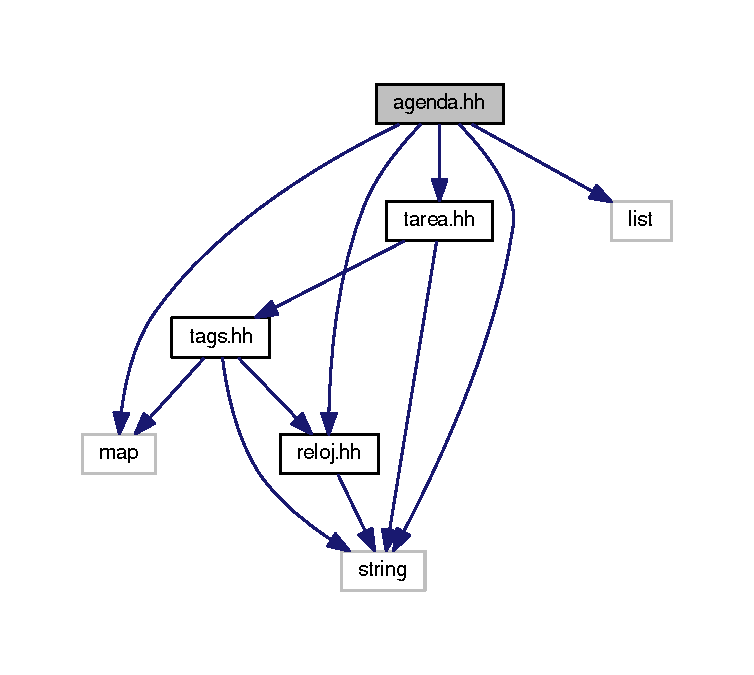
\includegraphics[width=211pt]{agenda_8hh__incl}
\end{center}
\end{figure}
\subsection*{Clases}
\begin{DoxyCompactItemize}
\item 
class \hyperlink{class_agenda}{Agenda}
\begin{DoxyCompactList}\small\item\em Representa una colección de Tareas, ordenadas por la hora de tarea. \end{DoxyCompactList}\end{DoxyCompactItemize}


\subsection{Descripción detallada}
Especificación de la clase \hyperlink{class_agenda}{Agenda}. 

Definición en el archivo \hyperlink{agenda_8hh_source}{agenda.\-hh}.


\hypertarget{comanda_8hh}{\section{Referencia del Archivo comanda.\-hh}
\label{comanda_8hh}\index{comanda.\-hh@{comanda.\-hh}}
}


Classe \hyperlink{class_comanda}{Comanda}.  


Dependencia gráfica adjunta para comanda.\-hh\-:\nopagebreak
\begin{figure}[H]
\begin{center}
\leavevmode
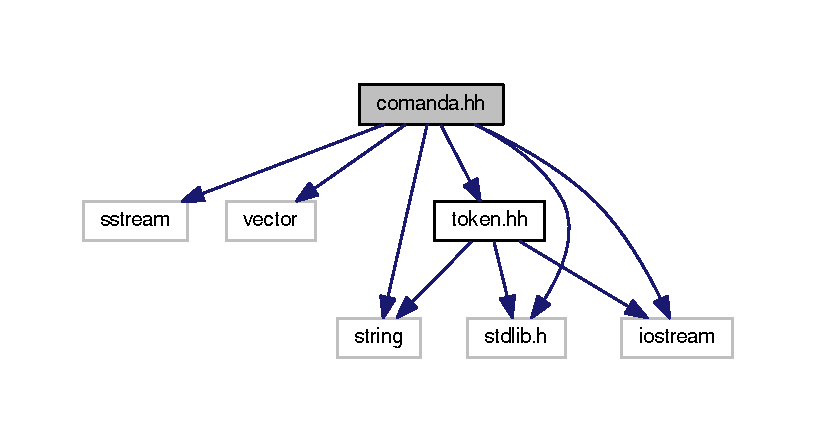
\includegraphics[width=350pt]{comanda_8hh__incl}
\end{center}
\end{figure}
\subsection*{Clases}
\begin{DoxyCompactItemize}
\item 
class \hyperlink{class_comanda}{Comanda}
\begin{DoxyCompactList}\small\item\em Representa una comanda (línia de text d'entrada). El mètode llegir permet utilitzar consultores sobre la comanda llegida i comprovar que no tingui errors sintàctics. \end{DoxyCompactList}\end{DoxyCompactItemize}


\subsection{Descripción detallada}
Classe \hyperlink{class_comanda}{Comanda}. 

Definición en el archivo \hyperlink{comanda_8hh_source}{comanda.\-hh}.


\hypertarget{pro2_8cc}{\section{Referencia del Archivo pro2.\-cc}
\label{pro2_8cc}\index{pro2.\-cc@{pro2.\-cc}}
}
Dependencia gráfica adjunta para pro2.\-cc\-:
\nopagebreak
\begin{figure}[H]
\begin{center}
\leavevmode
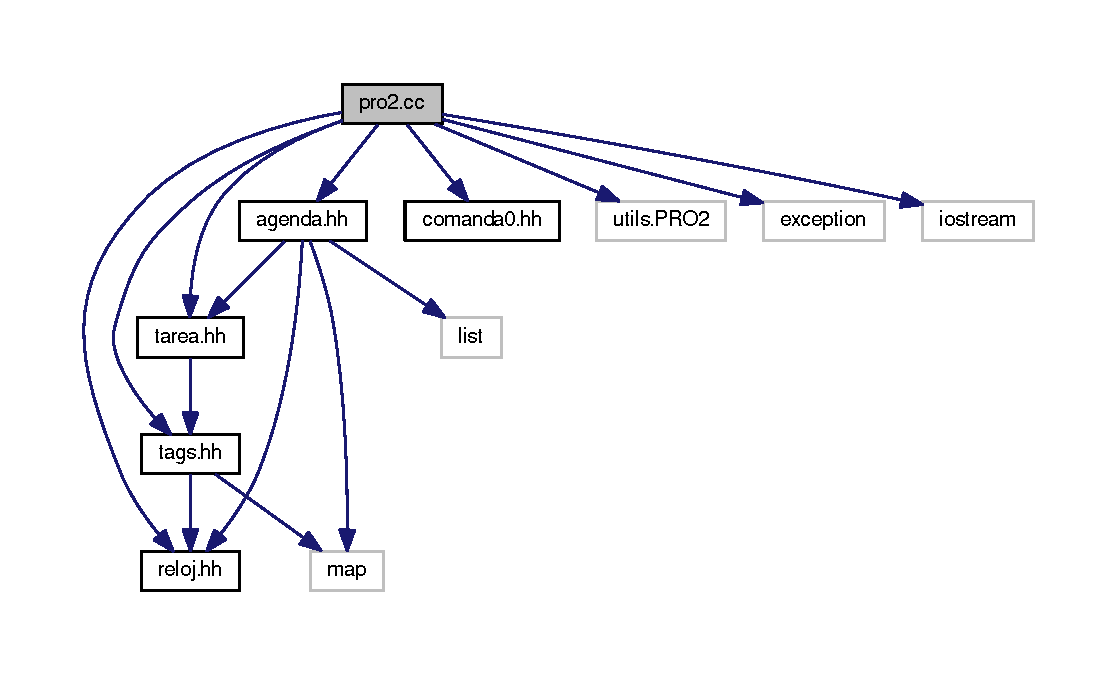
\includegraphics[width=350pt]{pro2_8cc__incl}
\end{center}
\end{figure}
\subsection*{Funciones}
\begin{DoxyCompactItemize}
\item 
int \hyperlink{pro2_8cc_ae66f6b31b5ad750f1fe042a706a4e3d4}{main} ()
\end{DoxyCompactItemize}


\subsection{Documentación de las funciones}
\hypertarget{pro2_8cc_ae66f6b31b5ad750f1fe042a706a4e3d4}{\index{pro2.\-cc@{pro2.\-cc}!main@{main}}
\index{main@{main}!pro2.cc@{pro2.\-cc}}
\subsubsection[{main}]{\setlength{\rightskip}{0pt plus 5cm}int main (
\begin{DoxyParamCaption}
{}
\end{DoxyParamCaption}
)}}\label{pro2_8cc_ae66f6b31b5ad750f1fe042a706a4e3d4}


Definición en la línea 8 del archivo pro2.\-cc.


\begin{DoxyCode}
9 \{
10     \hyperlink{class_comanda}{Comanda} c;
11     \hyperlink{class_agenda}{Agenda} a;
12     \textcolor{keywordtype}{bool} be = \textcolor{keyword}{false};
13     map<Reloj,Tarea> v;
14     \textcolor{keywordflow}{while}(c.\hyperlink{class_comanda_af2dbc8ccdbb94bed6ea26155edc71b57}{llegir}(be))\{
15         \textcolor{keywordtype}{bool} todo\_OK = \textcolor{keyword}{true};
16         \textcolor{keywordflow}{if}(not be)\{
17             \textcolor{keywordflow}{if}(c.\hyperlink{class_comanda_a847ee227fd7fea3a105dbd78735de453}{es\_consulta}())\{
18                 \hyperlink{class_reloj}{Reloj} r(\textcolor{stringliteral}{"00/00/00"});
19                 r.set\_hora(\textcolor{stringliteral}{"00:00"});
20                 \hyperlink{class_reloj}{Reloj} r2(\textcolor{stringliteral}{"31/12/99"});
21                 r.set\_hora(\textcolor{stringliteral}{"23:59"});
22                 \textcolor{keywordtype}{string} expr = \textcolor{charliteral}{'*'};
23                 \textcolor{keywordflow}{if}(c.\hyperlink{class_comanda_aadabfc85ec7cdeb45039e8952a1ab124}{nombre\_dates}()!=0 or c.\hyperlink{class_comanda_a81d17f4233e33f3baac7633546c066f0}{te\_expressio}() or c.
      \hyperlink{class_comanda_abf8b926146f3664aacfd24d7800014e5}{te\_hora}() or c.\hyperlink{class_comanda_a4280b6ae2d435d9c21bbed364cb1db3d}{nombre\_etiquetes}() != 0)\{
24                     \textcolor{keywordflow}{if}(c.\hyperlink{class_comanda_aadabfc85ec7cdeb45039e8952a1ab124}{nombre\_dates}() > 0 )\{
25                         \hyperlink{class_reloj}{Reloj} r(c.\hyperlink{class_comanda_ab4ce0a50bde32145d11cbaee753526c7}{data}(1));
26                         \hyperlink{class_reloj}{Reloj} r2(c.\hyperlink{class_comanda_ab4ce0a50bde32145d11cbaee753526c7}{data}(1));
27                         \textcolor{keywordflow}{if}(c.\hyperlink{class_comanda_aadabfc85ec7cdeb45039e8952a1ab124}{nombre\_dates}() == 2) r2.\hyperlink{class_reloj_a7afa0f35262ba2258a12b5cd739c0eca}{set\_fecha}(c.
      \hyperlink{class_comanda_ab4ce0a50bde32145d11cbaee753526c7}{data}(2));
28                         \textcolor{keywordflow}{if}(c.\hyperlink{class_comanda_abf8b926146f3664aacfd24d7800014e5}{te\_hora}())\{
29                             r.set\_hora(c.\hyperlink{class_comanda_ae8bca2ad702d3316dc1c53dcab7cac02}{hora}());
30                             r2.set\_hora(c.\hyperlink{class_comanda_ae8bca2ad702d3316dc1c53dcab7cac02}{hora}());
31                         \} \textcolor{keywordflow}{else} \{
32                             r.set\_hora(\textcolor{stringliteral}{"00:00"});
33                             r2.set\_hora(\textcolor{stringliteral}{"23:59"});
34                         \}
35                     \}
36                     \textcolor{keywordflow}{if}(c.\hyperlink{class_comanda_a81d17f4233e33f3baac7633546c066f0}{te\_expressio}()) expr = c.\hyperlink{class_comanda_aa3191131592fbf58d20bed1052c31cd1}{expressio}();
37                     \textcolor{keywordflow}{else} \textcolor{keywordflow}{if} (c.\hyperlink{class_comanda_a4280b6ae2d435d9c21bbed364cb1db3d}{nombre\_etiquetes}() == 1)\{ \textcolor{comment}{//TODO comprobar si se puede poner
       mas etiquetas}
38                         expr = c.\hyperlink{class_comanda_ac80e9a80d16c6bac9a134e431bca1ed0}{etiqueta}(1);
39                     \}
40                 \}
41                 v = a.\hyperlink{class_agenda_a82ce91d05bf272a3c0ead42fc64e84aa}{buscar\_tarea\_intervalo}(r,r2,expr);
42                 a.\hyperlink{class_agenda_a755177707be90968dedb6ff36647c3af}{imprimir\_menu}(v);
43             \} \textcolor{keywordflow}{else} \textcolor{keywordflow}{if} (c.\hyperlink{class_comanda_a2a33a5497c7d156f22065656cb48d9a1}{es\_modificacio}())\{
44                 \textcolor{comment}{// Pre: se ha realizado una consulta anteriormente}
45                 \textcolor{keywordtype}{int} tasca = c.\hyperlink{class_comanda_a67591051e9c5977c324ad8f8c3ac16e3}{tasca}();
46 
47                 map<Reloj,Tarea>::iterator it(v.begin());
48                 advance(i1,tasca); \textcolor{comment}{// selecionamos la tarea}
49                 \hyperlink{class_reloj}{Reloj} r1 = it->first;
50                 \hyperlink{class_reloj}{Reloj} r2 = it->first;
51                 \hyperlink{class_tarea}{Tarea} t = it->second;
52                 \textcolor{keywordflow}{if}(c.\hyperlink{class_comanda_a5452f5a877d58627cd2bd871cf31b074}{te\_titol}())\{
53                     t.\hyperlink{class_tarea_aa9371098468f9074182b5df5dc240fc3}{set\_titulo}(c.\hyperlink{class_comanda_ad1cefdda3db389d9ab536a59e2ee907d}{titol}());
54                 \}
55                 \textcolor{keywordflow}{if}(c.\hyperlink{class_comanda_abf8b926146f3664aacfd24d7800014e5}{te\_hora}())\{
56                     r2.\hyperlink{class_reloj_a644b36309ac37e113bf804321d5629dd}{set\_hora}(c.\hyperlink{class_comanda_ae8bca2ad702d3316dc1c53dcab7cac02}{hora}());
57                 \}
58                 \textcolor{keywordflow}{if}(c.\hyperlink{class_comanda_aadabfc85ec7cdeb45039e8952a1ab124}{nombre\_dates}() != 0)\{
59                     r2.\hyperlink{class_reloj_a7afa0f35262ba2258a12b5cd739c0eca}{set\_fecha}(c.\hyperlink{class_comanda_ab4ce0a50bde32145d11cbaee753526c7}{data}(1));
60                 \}
61                 todo\_OK = a.\hyperlink{class_agenda_aecbb7c1af5d9816012ba9b6b7c5f3bfe}{modificar\_tarea}(r1,r2,t);
62 
63 
64             \} \textcolor{keywordflow}{else} \textcolor{keywordflow}{if} (c.\hyperlink{class_comanda_a614467bedacc9cf29cc5a9dcbba6b23d}{es\_insercio}())\{
65                 \hyperlink{class_reloj}{Reloj} r;
66                 \textcolor{keywordflow}{if}(c.\hyperlink{class_comanda_aadabfc85ec7cdeb45039e8952a1ab124}{nombre\_dates}() == 1)\{
67                     r.\hyperlink{class_reloj_a7afa0f35262ba2258a12b5cd739c0eca}{set\_fecha}(c.\hyperlink{class_comanda_ab4ce0a50bde32145d11cbaee753526c7}{data}(1));
68                 \} \textcolor{keywordflow}{else} \{
69                     r = a.\hyperlink{class_agenda_aba4ae16c8c68b5b08adabd6d3c633630}{get\_RelojActual}();
70                 \}
71                 r.\hyperlink{class_reloj_a644b36309ac37e113bf804321d5629dd}{set\_hora}(c.\hyperlink{class_comanda_ae8bca2ad702d3316dc1c53dcab7cac02}{hora}());
72                 \hyperlink{class_tags}{Tags} tags;
73                 \textcolor{keywordflow}{if}(c.\hyperlink{class_comanda_a4280b6ae2d435d9c21bbed364cb1db3d}{nombre\_etiquetes}() != 0)\{
74                     \textcolor{keywordflow}{for}(\textcolor{keywordtype}{int} i = 1; i <= c.\hyperlink{class_comanda_a4280b6ae2d435d9c21bbed364cb1db3d}{nombre\_etiquetes}() ; ++i)\{
75                         tags.\hyperlink{class_tags_a0bbd998942d9415108eae2be28daedd0}{add\_tag}(c.\hyperlink{class_comanda_ac80e9a80d16c6bac9a134e431bca1ed0}{etiqueta}(i));
76                     \}
77                 \}
78 
79                 \hyperlink{class_tarea}{Tarea} tarea(c.\hyperlink{class_comanda_ad1cefdda3db389d9ab536a59e2ee907d}{titol}(),tags);
80                 todo\_OK = a.\hyperlink{class_agenda_aeba776d0394a5cc0da53e7955d713133}{anadir\_tarea}(r,tarea);
81 
82 
83             \} \textcolor{keywordflow}{else} \textcolor{keywordflow}{if} (c.\hyperlink{class_comanda_aa8767f298317c3bb07f90676cabb8c43}{es\_rellotge}())\{
84                 \hyperlink{class_reloj}{Reloj} r;
85                 \textcolor{keywordflow}{if}(not c.\hyperlink{class_comanda_abf8b926146f3664aacfd24d7800014e5}{te\_hora}() and not c.\hyperlink{class_comanda_aadabfc85ec7cdeb45039e8952a1ab124}{nombre\_dates}() != 0)\{
86                     \textcolor{keywordflow}{if}(c.\hyperlink{class_comanda_abf8b926146f3664aacfd24d7800014e5}{te\_hora}()) r.\hyperlink{class_reloj_a644b36309ac37e113bf804321d5629dd}{set\_hora}(c.\hyperlink{class_comanda_ae8bca2ad702d3316dc1c53dcab7cac02}{hora}());
87                     \textcolor{keywordflow}{if}(c.\hyperlink{class_comanda_aadabfc85ec7cdeb45039e8952a1ab124}{nombre\_dates}() != 0) r.\hyperlink{class_reloj_a7afa0f35262ba2258a12b5cd739c0eca}{set\_fecha}(c.
      \hyperlink{class_comanda_ab4ce0a50bde32145d11cbaee753526c7}{data}(1));
88                     todo\_OK = a.\hyperlink{class_agenda_a8faca3490d5b520615c99809ce80521d}{set\_Reloj}(r);
89                 \} \textcolor{keywordflow}{else} \{ \textcolor{comment}{// caso consulta}
90                     r = a.\hyperlink{class_agenda_aba4ae16c8c68b5b08adabd6d3c633630}{get\_RelojActual}();
91                     cout << r.get\_fecha() << \textcolor{stringliteral}{"   "} << r.get\_hora() << endl;
92                 \}
93             \} \textcolor{keywordflow}{else} \textcolor{keywordflow}{if} (c.\hyperlink{class_comanda_a1f435f8b605f0d1f5cbb06c8c6fe4005}{es\_passat}())\{
94                 \hyperlink{class_reloj}{Reloj} reloj1(\textcolor{stringliteral}{"00.00.00"},\textcolor{stringliteral}{"00:00"});
95                 \hyperlink{class_reloj}{Reloj} reloj2 = a.\hyperlink{class_agenda_aba4ae16c8c68b5b08adabd6d3c633630}{get\_RelojActual}();
96                 \textcolor{keywordtype}{string} expr = \textcolor{charliteral}{'*'};
97                 v = a.\hyperlink{class_agenda_a82ce91d05bf272a3c0ead42fc64e84aa}{buscar\_tarea\_intervalo}(reloj1,reloj2,expr);
98                 a.\hyperlink{class_agenda_a755177707be90968dedb6ff36647c3af}{imprimir\_menu}(v);
99             \} \textcolor{keywordflow}{else} \{ \textcolor{comment}{//esborrat}
100                 \textcolor{keywordtype}{string} tipus = c.\hyperlink{class_comanda_a998dc172668a108837512f818ca5430f}{tipus\_esborrat}();
101                 \textcolor{comment}{// Pre: se ha realizado una consulta anteriormente}
102                 \textcolor{keywordtype}{int} tasca = c.\hyperlink{class_comanda_a67591051e9c5977c324ad8f8c3ac16e3}{tasca}();
103 
104                 map<Reloj,Tarea>::iterator it(v.begin());
105                 advance(i1,tasca); \textcolor{comment}{// selecionamos la tarea}
106                 \hyperlink{class_reloj}{Reloj} r1 = it->first;
107                 \hyperlink{class_reloj}{Reloj} r2 = it->first;
108                 \hyperlink{class_tarea}{Tarea} t = it->second;
109 
110                 \textcolor{keywordflow}{if}(tipus == \textcolor{stringliteral}{"etiquetes"})\{
111                     \hyperlink{class_tags}{Tags} tags;
112                     t.\hyperlink{class_tarea_a70871ce092aceb665b59f2094520bba4}{set\_tags}(tags);
113                     todo\_OK = a.\hyperlink{class_agenda_aecbb7c1af5d9816012ba9b6b7c5f3bfe}{modificar\_tarea}(r1,r2,t);
114                 \} \textcolor{keywordflow}{else} \textcolor{keywordflow}{if}(tipus == \textcolor{stringliteral}{"etiqueta"})\{
115                     t.\hyperlink{class_tarea_a7c92a7021f2b2ef18092e4a9bb27b24d}{borar\_tag}(c.\hyperlink{class_comanda_ac80e9a80d16c6bac9a134e431bca1ed0}{etiqueta}(1));
116                     todo\_OK = a.\hyperlink{class_agenda_aecbb7c1af5d9816012ba9b6b7c5f3bfe}{modificar\_tarea}(r1,r2,t);
117                 \} \textcolor{keywordflow}{else} \{ \textcolor{comment}{// Borrar tarea}
118                     todo\_OK = a.\hyperlink{class_agenda_af1d7e74d388a0b22c8186b4b329d0bae}{borrar\_tarea}(r1,t);
119                 \}
120 
121             \}
122 
123         \textcolor{keywordflow}{if}(not todo\_OK) cout << \textcolor{stringliteral}{"No s'ha realitzat"} << endl;
124 
125         \}
126     \}
127 \}
\end{DoxyCode}

\hypertarget{reloj_8hh}{\section{Referencia del Archivo reloj.\-hh}
\label{reloj_8hh}\index{reloj.\-hh@{reloj.\-hh}}
}


Clase \hyperlink{class_reloj}{Reloj}.  


Dependencia gráfica adjunta para reloj.\-hh\-:
\nopagebreak
\begin{figure}[H]
\begin{center}
\leavevmode
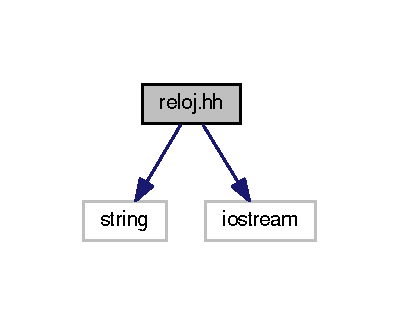
\includegraphics[width=126pt]{reloj_8hh__incl}
\end{center}
\end{figure}
\subsection*{Clases}
\begin{DoxyCompactItemize}
\item 
class \hyperlink{class_reloj}{Reloj}
\begin{DoxyCompactList}\small\item\em Representa el reloj interno. \end{DoxyCompactList}\end{DoxyCompactItemize}


\subsection{Descripción detallada}
Clase \hyperlink{class_reloj}{Reloj}. 

Definición en el archivo \hyperlink{reloj_8hh_source}{reloj.\-hh}.


\hypertarget{tags_8hh}{\section{Referencia del Archivo tags.\-hh}
\label{tags_8hh}\index{tags.\-hh@{tags.\-hh}}
}


Especificación de la clase Tag.  


Dependencia gráfica adjunta para tags.\-hh\-:\nopagebreak
\begin{figure}[H]
\begin{center}
\leavevmode
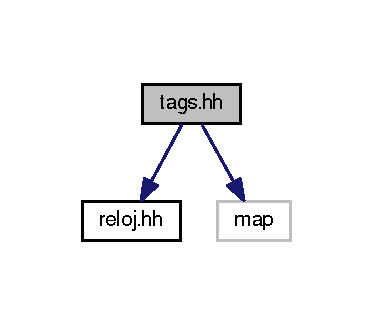
\includegraphics[width=208pt]{tags_8hh__incl}
\end{center}
\end{figure}
\subsection*{Clases}
\begin{DoxyCompactItemize}
\item 
class \hyperlink{class_tags}{Tags}
\begin{DoxyCompactList}\small\item\em Representa una colección de etiquetas. \end{DoxyCompactList}\end{DoxyCompactItemize}


\subsection{Descripción detallada}
Especificación de la clase Tag. 

Definición en el archivo \hyperlink{tags_8hh_source}{tags.\-hh}.


\hypertarget{tarea_8hh}{\section{Referencia del Archivo tarea.\-hh}
\label{tarea_8hh}\index{tarea.\-hh@{tarea.\-hh}}
}
Dependencia gráfica adjunta para tarea.\-hh\-:\nopagebreak
\begin{figure}[H]
\begin{center}
\leavevmode
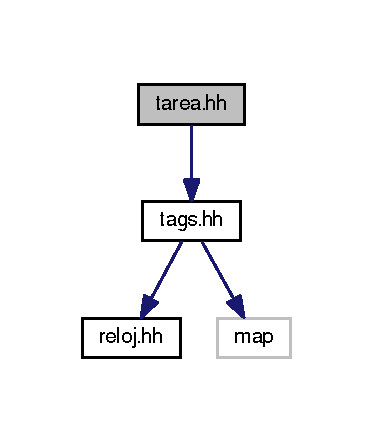
\includegraphics[width=208pt]{tarea_8hh__incl}
\end{center}
\end{figure}
\subsection*{Clases}
\begin{DoxyCompactItemize}
\item 
class \hyperlink{class_tarea}{Tarea}
\begin{DoxyCompactList}\small\item\em Representa una tarea, con título y 0 o más etiquetas. \end{DoxyCompactList}\end{DoxyCompactItemize}

\hypertarget{token_8hh}{\section{Referencia del Archivo token.\-hh}
\label{token_8hh}\index{token.\-hh@{token.\-hh}}
}


Classe \hyperlink{class_token}{Token}.  


Dependencia gráfica adjunta para token.\-hh\-:\nopagebreak
\begin{figure}[H]
\begin{center}
\leavevmode
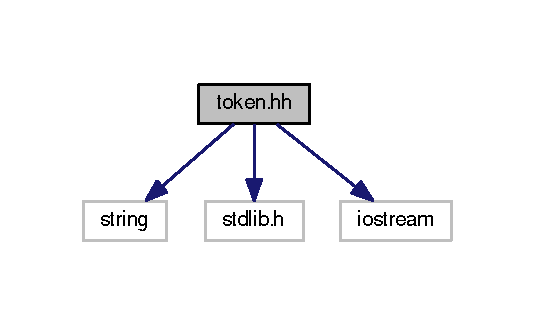
\includegraphics[width=256pt]{token_8hh__incl}
\end{center}
\end{figure}
\subsection*{Clases}
\begin{DoxyCompactItemize}
\item 
class \hyperlink{class_token}{Token}
\begin{DoxyCompactList}\small\item\em Representa un string rellevant per a la classe \hyperlink{class_comanda}{Comanda}. \end{DoxyCompactList}\end{DoxyCompactItemize}


\subsection{Descripción detallada}
Classe \hyperlink{class_token}{Token}. 

Definición en el archivo \hyperlink{token_8hh_source}{token.\-hh}.


\addcontentsline{toc}{part}{Índice}
\printindex
\end{document}
